\chapter{Analysis Strategy}

The analysis aims at observing triboson production of $\PZ\PZ\PGg$ and $\PW\PZ\PGg$, by combining three orthogonal channels.
The \textit{channels} are defined based on the number of loose leptons (Sections \ref{sec:ele_selection} and \ref{sec:muo_selection}) in the event.
Each channel is further divided into several \textit{regions}, based on the number of leptons that pass the tight selection,
and whether or not there is a photon that passes the tight selection (Section \ref{sec:photonID}).
The full scope of the division is illustrated in Table \ref{tab:region_definition}.

\begin{table}
  \caption{Definition of the analysis division into channels and regions.}
  \label{tab:region_definition}
  \resizebox{\textwidth}{!}{%
    \begin{tabular}{|c | c|c|c | c|c|c|c | c|}
      \hline
      channel $\rightarrow$    & \multicolumn{3}{c|}{4 \Pl} & \multicolumn{4}{c|}{3 \Pl $\ (\ptmiss > 30 \GeV)$} & 2 \Pl   \\
      \hline
      \Pl status $\rightarrow$ & 4P      & 3P1F & 2P2F      & 3P      & 2P1F & 2P2F & 3F                        & 2P      \\
      \hline
      \PGg PASS                & \cellcolor[HTML]{cc7fff}SR & \multirow{2}*{CR \Pl} & \multirow{2}*{CR \Pl} &
                                 \cellcolor[HTML]{a4c2f3}SR & \multirow{2}*{CR \Pl} & \multirow{2}*{CR \Pl} & \multirow{2}*{CR \Pl}  &
                                 \cellcolor[HTML]{ffcb7f}SR \\
      \cline{1-2} \cline{5-5} \cline{9-9}
      \PGg FAIL                & CR \PGg &      &           & CR \PGg &      &      &                           & CR \PGg \\
      \hline %% \midrule
      \multicolumn{3}{c}{}                                & & \multicolumn{4}{c|}{3 \Pl $\ (\ptmiss < 30 \GeV)$} & \multicolumn{1}{c}{} \\
      \cline{5-8}
      \multicolumn{3}{c}{}                                & & 3P & 2P1F & 1P2F & 3F                             & \multicolumn{1}{c}{} \\
      \cline{5-8}
      \multicolumn{3}{c}{}                                & & \multicolumn{2}{c|}{\shortstack[c]{\vspace{.5ex} \\ \Pl-FR and \PGg-FR \\ measurement}} & & & \multicolumn{1}{c}{} \\
      \cline{5-8}
    \end{tabular}
  }
\end{table}

The 4\Pl channel targets $\PZ\PZ\PGg$ production with fully leptonic decay of the two Z bosons.
The 3\Pl channel focuses primarily on $\PW\PZ\PGg$, also with fully leptonic decay of the \PW and \PZ bosons,
but since there is a small contamination of $\PZ\PZ\PGg$ it benefits from a combined fit of the two.
Finally, the 2\Pl channel targets both $\PZ\PZ\PGg$ and $\PW\PZ\PGg$, where one \PZ decays to leptons,
and the other massive boson decays to quarks, which hadronize to jets.

\section{Signal}
\label{sec:signal}
This analysis searches for the simultaneous production of two massive bosons and a photon in a single hard scattering of a proton-proton collision at 13\TeV.
The signature of these processes varies among the three channels, but includes a number of high-momentum, isolated leptons,
with one or two pairs resonating to the Z boson mass,
and an isolated photon with high momentum.

However, there is a degree of ambiguity in what can be considered triboson production when a photon is present in the final state.
For example, in the four lepton channel, the reaction
$p p \to 4 \Pl \PGg$
has three contributions:
\begin{enumerate}
\item The photon comes from an initial state fermion (Figure \ref{fig:ppTo4LG_hard})
\item The photon comes from a Triple or Quartic Gauge Coupling (e.g. Figure \ref{fig:ppTo4LG_GC})
\item The photon is emitted as Final State Radiation (FSR) by one of the leptons from the decay of a \PZ (e.g. Figure \ref{fig:ppTo4LG_FSR})
\end{enumerate}

This analysis considers only the first and the second processes as the signal.
The third process, even though it has exactly the same particles in the final state, is part of the irreducible backgrounds.

Note that in the SM only $\PW\PZ\PGg$ can be produced via TGA/QGC

However, results will be reported both including and excluding the third contribution, by means of an additional dedicated cut described in Section \ref{sec:FSR_cut}.

\begin{figure}
  \centering
  \subfigure [From initial-state fermion] {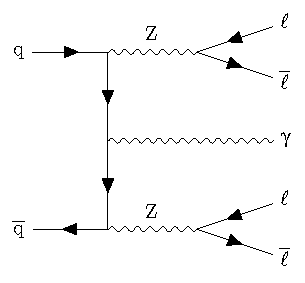
\includegraphics[width=.319\textwidth]{triboson_4LG.pdf} \label{fig:ppTo4LG_hard}}
  \subfigure [Non-abelian coupling]       {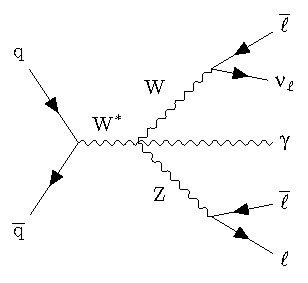
\includegraphics[width=.319\textwidth]{QGC_3LNuG.pdf}    \label{fig:ppTo4LG_GC}  }
  \subfigure [From final-state fermion]   {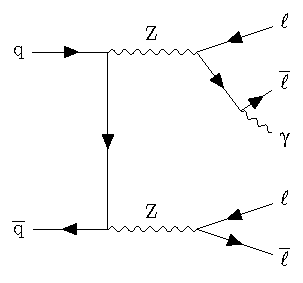
\includegraphics[width=.319\textwidth]{ZZ_4LG.pdf}       \label{fig:ppTo4LG_FSR} }
\caption{Standard Model processes that yield four isolated leptons and a photon in the final state.}
\label{fig:ppTo4LG}
\end{figure}

Similarly, in the three lepton channel, only photons from the hard scattering or the ISR are part of the signal definition,
while contributions from FSR photons from one of the three leptons are part of the irreducible backgrounds.

\subsection{Signal defintion and simulation}
\note{This draft is to be checked}
The cut on the minimum \DR{} distance between the photon and the signal leptons (see Section \ref{sec:evt_photon_selection})
aims to exclude the FSR contribution.
However, a small fraction of events where the photon is emitted at large angle remains. \note{Are we sure?}

\section{Backgrounds}

An accurate description of the background process is an essential aspect of any analysis since it affects the extraction of signal yields.
The main background sources differ between the three channels, but generally belong to the category of \textit{reducible background}.
This class contains processes which have a different final state from the signal.
However, either due to additional particles produced in combination which may produce a different signature in the detector,
other collisions in the same bunch crossing (pileup),
or other errors in the reconstruction procedure,
they produce events which may erroneously pass the selection.
Often these backgrounds prove difficult to model in simulation,
and it becomes advisable to use a data-driven method for their estimation.

The other category comprises \textit{irreducible backgrounds},
which are processes that generate a final state with the same particles as the signal,
although the kinematic distributions may be different.
Usually processes in this class are estimated with simulation,
but in some cases it is possible to constrain their normalisation in a control region.

%% \subsection{Four lepton channel}
For the 4\Pl channel the predominant background component is the production of two on-shell \PZ bosons
and a photon that is either radiated as FSR from one of the leptons
or from a misreconstructed jet.
As described in Section \ref{sec:simulation}, it can be either produced from two quarks,
or proceed from a gluon initiated loop.
Additional backgrounds such as $\PQt\PAQt\PZ$ and VVV (V = \PZ, \PW) result in very small contributions.

%% \subsection{Three lepton channel}
In the 3\Pl channel the main background contributions are Drell-Yan + jets, $\PZ\PGg$ + jets
and $\PW\PZ$ plus a photon that is either radiated as FSR from one of the leptons or from a misreconstructed jet.
Another significant contribution comes from $\PZ\PZ \to 4\Pl$ where one of the leptons is lost or misreconstructed as a photon.
There is also a small fraction of events from $\PZ\PZ\PGg$ in which one of the leptons is outside the detector acceptance. \todo{should check in MC}
Additional backgrounds from rare processes such as $\PQt\PAQt\PZ$ and VVV (V = \PZ, \PW) result in very small contributions and are estimated with simulation.

\paragraph{Reducible background\\}
This group of backgrounds arises from processes in which some of the reconstructed leptons or photons do not correspond to real, prompt leptons from the vector bosons decay or photons from the hard process.
This particles can either be \nonprompt leptons or photons, or misidentified light-flavour jets.

\Nonprompt leptons come mainly from decays of heavy flavour mesons and electrons from asymmetric photons conversions,
while \nonprompt photons originate primarily from decays of light neutral mesons like \PGpz or \PGh.
Both leptons and photons in this category tend to be non-isolated from the nearby jet activity.

The other class is comprised of misidentified jets, mostly from light-flavour quarks, which can erroneously be reconstructed as either leptons,
if a track is associated to the main energy deposits, or as photons otherwise.
These misidentified photons tend to have a different energy distribution in the ECAL with respect to real photons,
which makes shower shape variables effective in separating this background from real photons.

In the following the terms \textit{fake leptons} and \textit{fake photons} are used to refer to both \nonprompt and misidentified objects.

\todo{Look in Wgamma or some other analysis more detail about nonprompt/misidentified photons}

\subsection{Fake Leptons}
To estimate the expected fake lepton background yield in the signal region,
dedicated control regions are defined with requirements similar to the signal region but in such a way not to contain signal events.
To enhance the \nonprompt lepton component, events in these regions are required to
have a number of leptons that fail the tight selection, while passing the loose criteria.
The other selections are identical to maintain similarity with the signal region.

The fake lepton background yield in the signal region is extrapolated from these regions
according to the probability for loose lepton candidates to pass also the final selection criteria (defined in Section 4.1.2).
These probabilities, referred to as fake rates, are estimated independently as illustrated in the following section.

\paragraph{Four lepton channel\\}
For the 4\Pl channel, two control regions are defined.
The former, named CR3P1F, one of the leptons of the $\PZ_2$ must fail the tight selection,
while the other three (2 from $\PZ_1$ and the other from $\PZ_2$) must pass the tight identification and isolation criteria.
It is expected to be populated by $\PW\PZ$, with contributions from Drell-Yan and $\PZ\PGg$,
along with a fraction of events from $(\PQq\PAQq/\Pg\Pg) \to \PZ\PZ$ where one of the prompt leptons fails the selection.

In the latter region, named CR2P2F, both leptons from the $\PZ_2$ fail the tight selection, while the leptons of the $\PZ_1$ pass the tight criteria.
This region is populated primarily by Drell-Yan events, with contributions from $\PZ\PGg$ and $\PQt\PAQt+X$.

This method was used by several analyses targeting a final state with four leptons from $\PZ\PZ$ decay~\cite{CMS-SMP-16-001, CMS-SMP-17-006, CMS-SMP-20-001, CMS-PAS-SMP-22-001},
and is described in detail in Reference~\cite{CMS-HIG-13-002} as the ``Method using opposite-sign (OS) leptons''.

\paragraph{Three lepton channel\\}
\note{At the moment, the data-driven fake estimate does NOT work in SR3P. Maybe we shouldn't discuss it if we don't use it.}

\note{SMP-16-002~\cite{SMP-16-002} (2015 data) uses a dijet region to measure the fake rate:
\textit{``The misidentification probability is measured from a sample of
dijet events enriched in nonprompt leptons. The sample is selected
with one jet passing the relaxed lepton identification requirements
matched to a single lepton trigger, defined as the probe lepton.''}}

\note{SMP-20-014~\cite{SMP-20-014} (full Run2) uses a L+j region:
\textit{``This CR is defined by requiring a single lepton with pT greater than 10 GeV, and at least
a reconstructed jet that is well separated from the lepton at $\DR(\PGg, j) > 0.7$. Contributions from
EWK processes are subtracted to obtain a pure nonprompt measurement region.''}}

\todo{Describe fake leptons method in 3L channel}

\subsubsection{Lepton fake rate measurement}
The measurement of the lepton fake rate, which is the probability that a fake lepton that passes the loose selection also passes the tight criteria,
is carried out in a separate control region which is enriched in contempt leptons.

This region, denoted as $\PZ+L$, is defined as containing a valid \PZ candidate whose leptons must have $\pt^{\Pl_{Z,1}} > 20 \GeV$ and $\pt^{\Pl_{Z,2}} > 10 \GeV$
and an additional lepton which passes the loose selection.
Additionally, the \PZ candidate must have a mass within 10 \GeV from the nominal peak,
and the missing energy must be $\MET < 20 \GeV$ to reduce the contribution from real leptons from $\PW\PZ$.
The last requirement means that this region is orthogonal to all of the regions in the 3\Pl channel, in which the MET is required to be greater than 30 \GeV.

The fake rate is measured on the third lepton in several bins of transverse momentum, separately for the barrel and endcap and flavour.
The measurement is done for each year of data taking, and the resulting rates can be seen in Figure \ref{fig:leptonFR}.

\begin{figure}
  \centering
  \subfigure [2016] {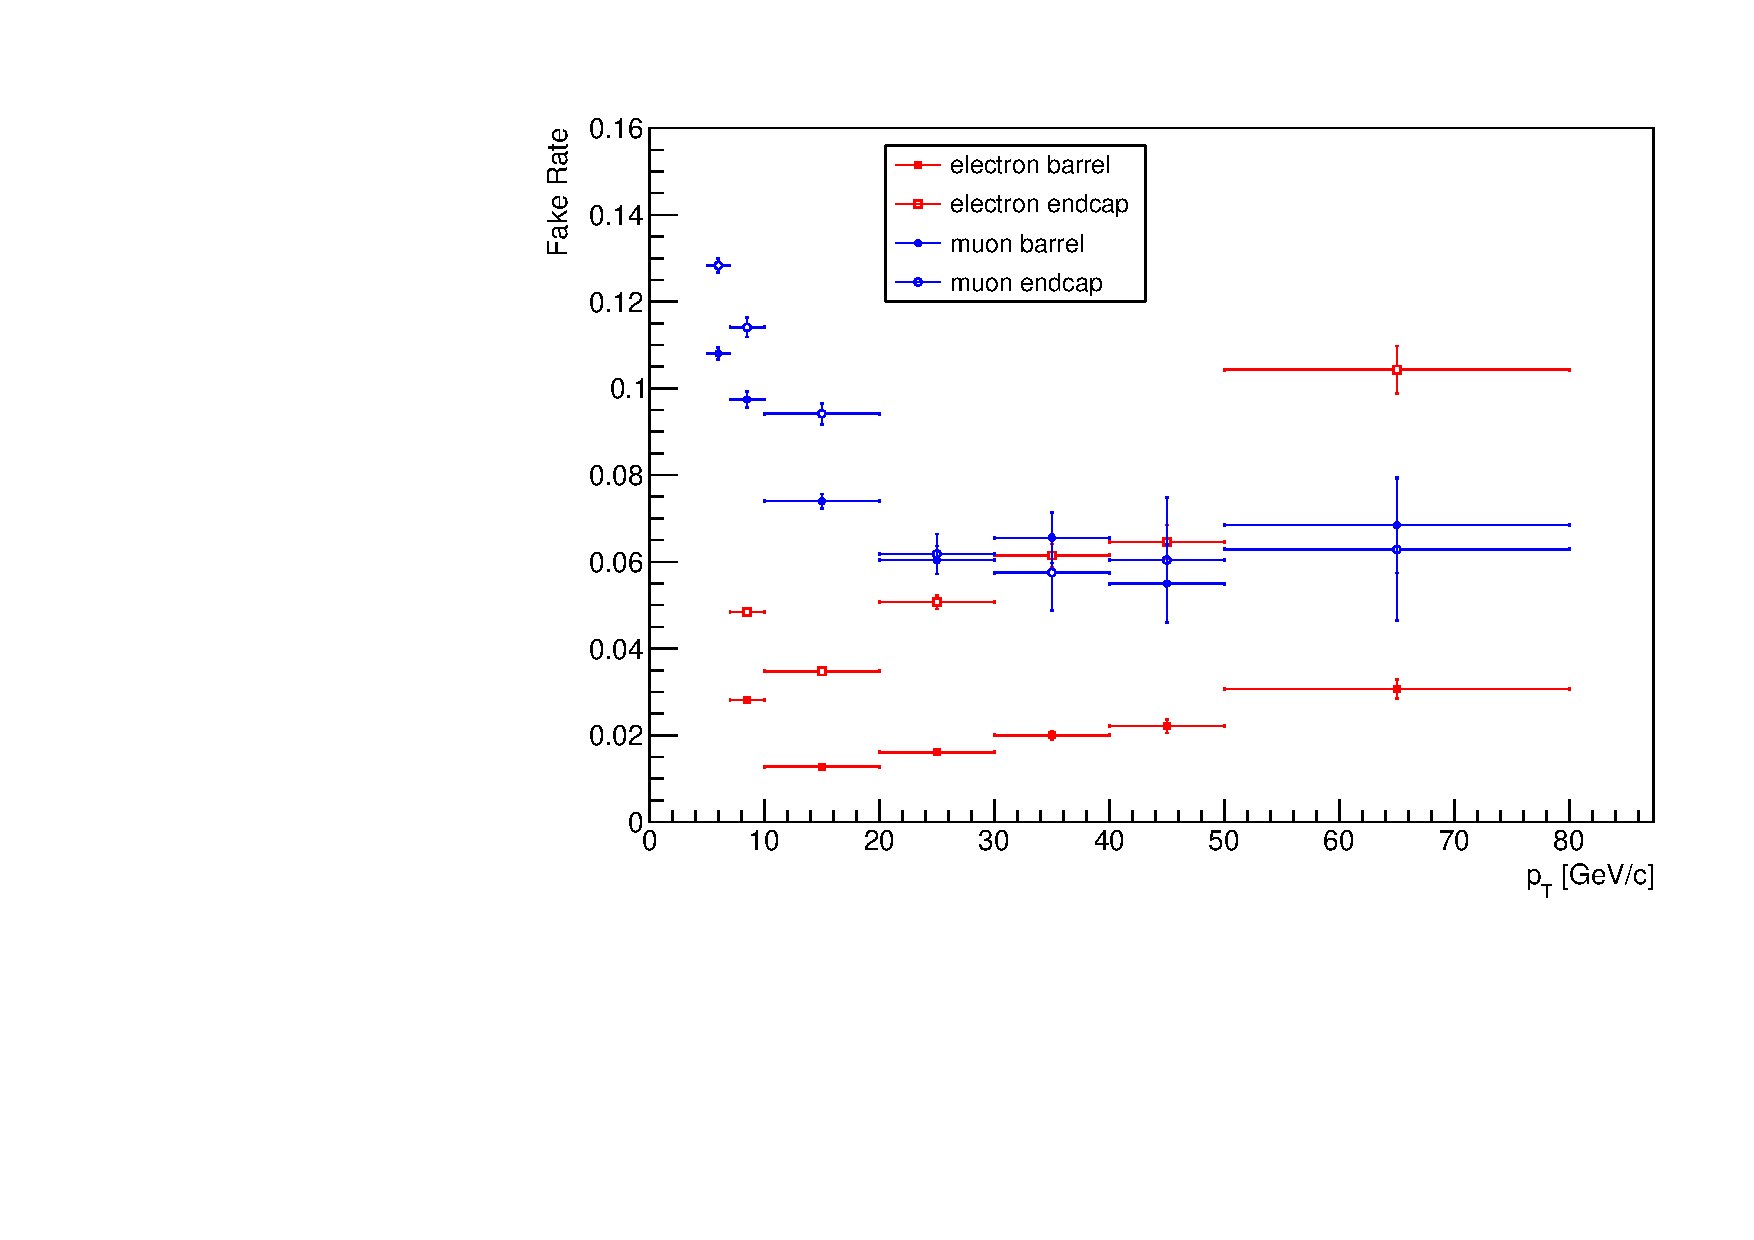
\includegraphics[width=.5\textwidth]{leptonFakeRate_2016.pdf}}%
  \subfigure [2017] {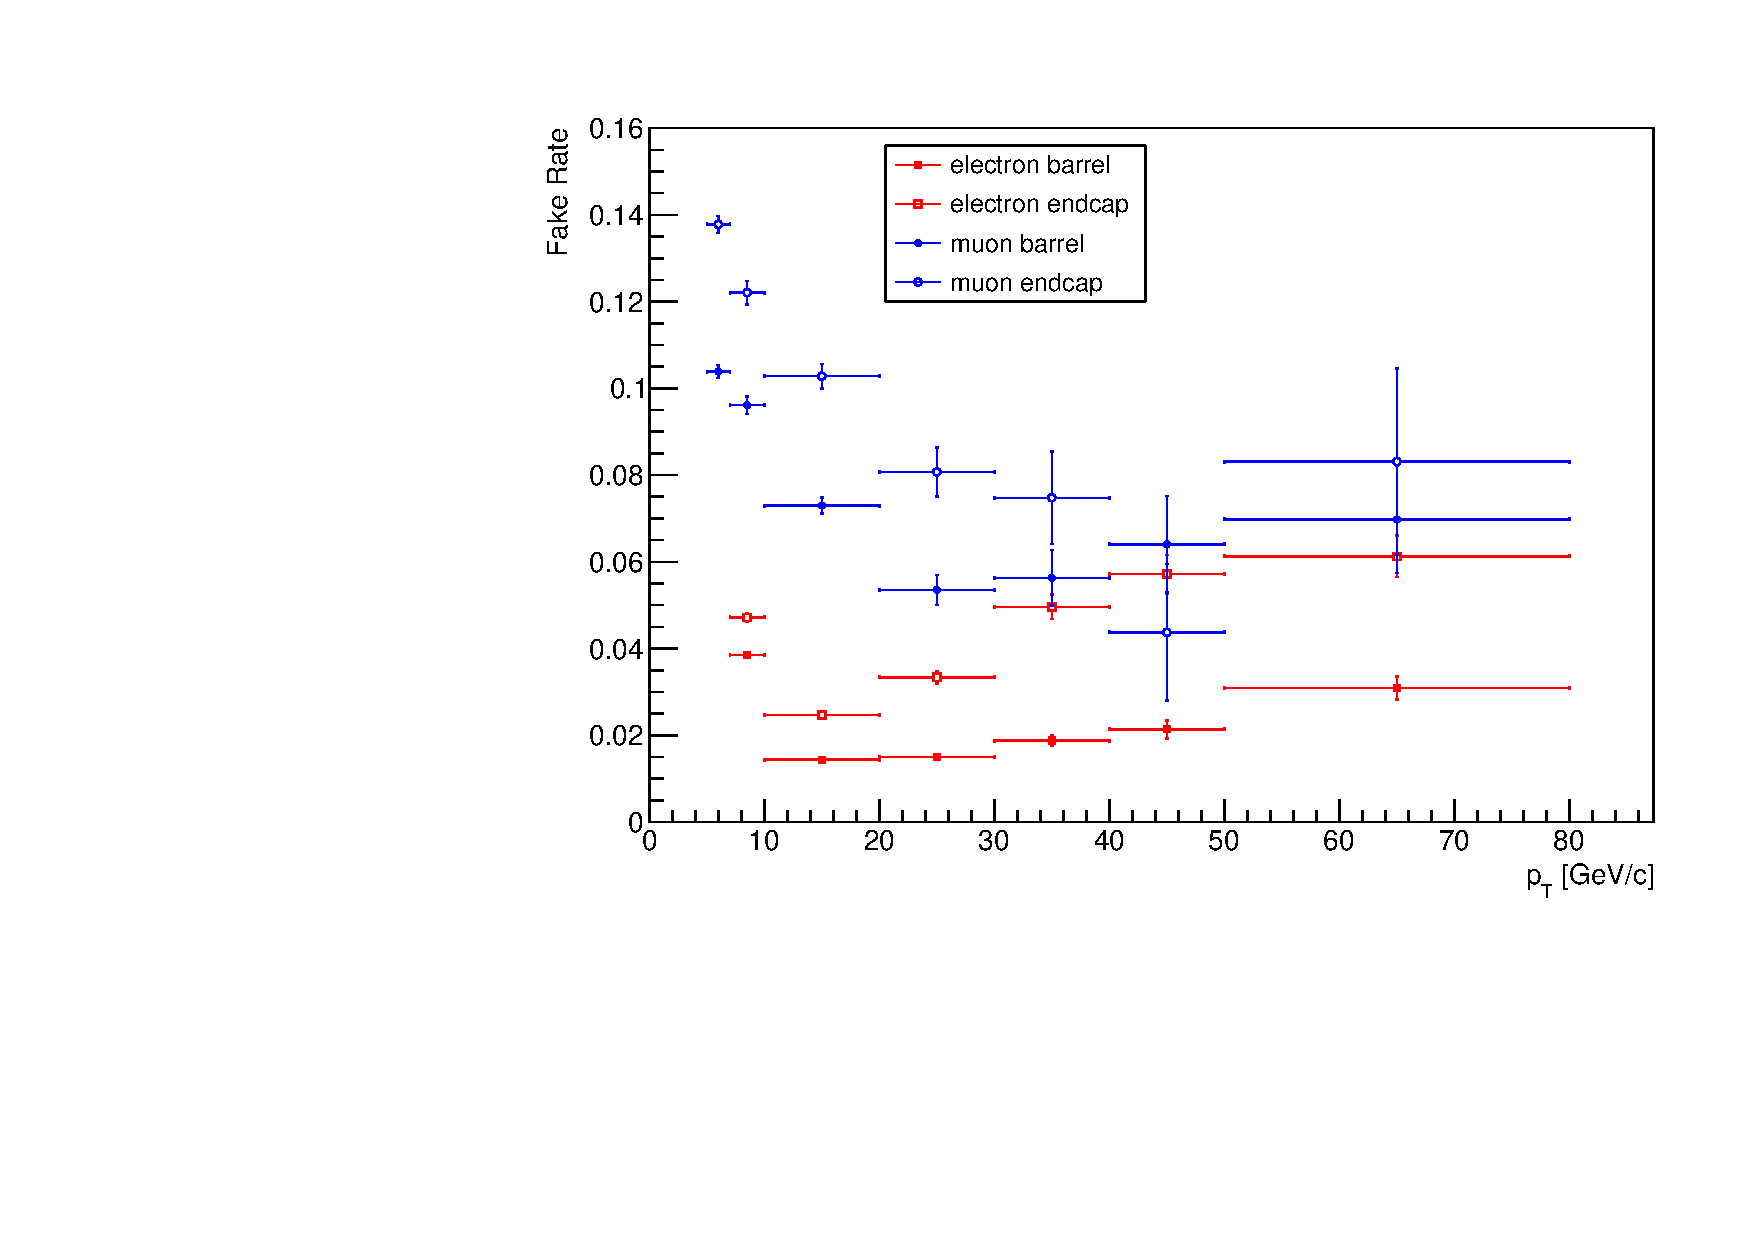
\includegraphics[width=.5\textwidth]{leptonFakeRate_2017.pdf}}\\
  \subfigure [2018] {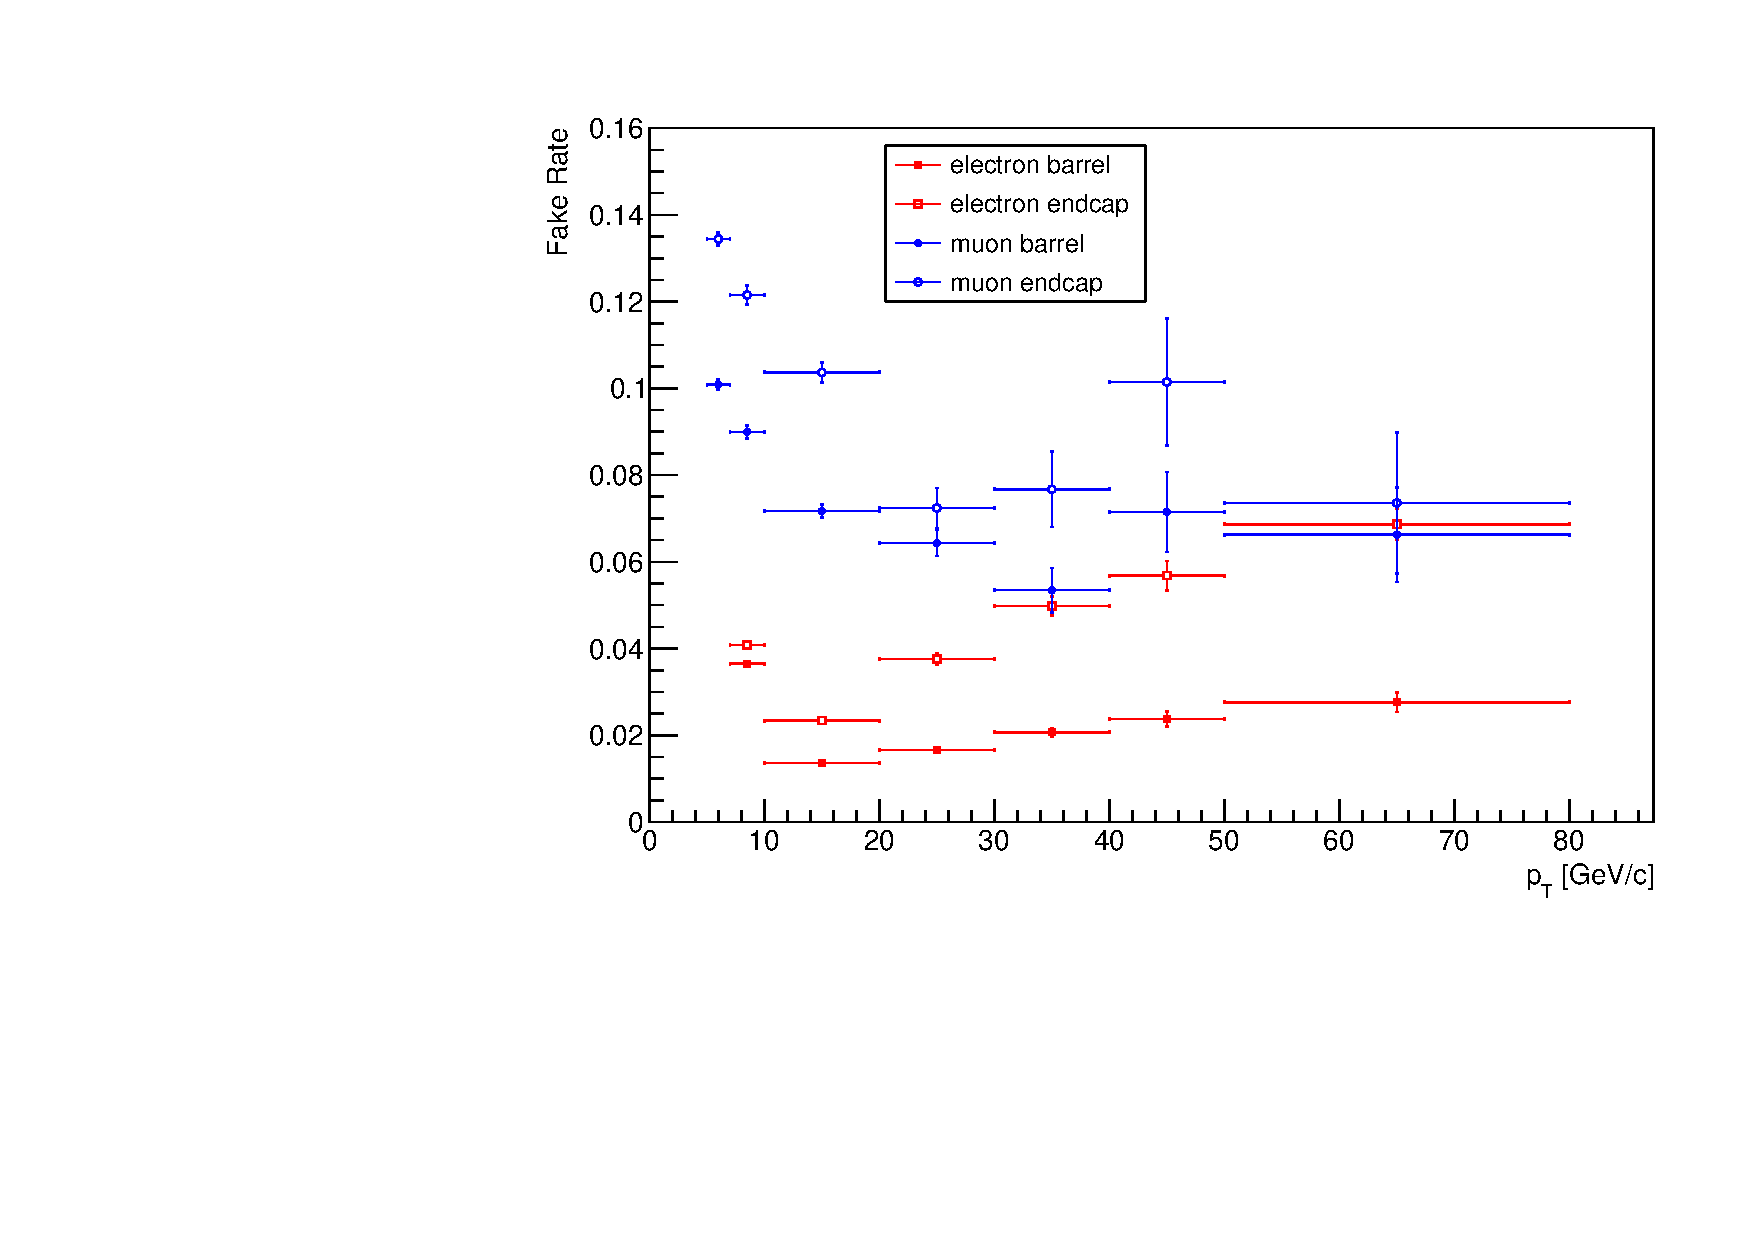
\includegraphics[width=.5\textwidth]{leptonFakeRate_2018.pdf}}
  \caption{Lepton fake rates measured in the $\PZ+L$ control region, for each year of data-taking.}
  \label{fig:leptonFR}
\end{figure}

The uncertainty on the fake lepton background estimation arises from the difference in composition of the
background processes in the region where the fake rate is measured and where it is applied.
This uncertainty was measured by several analyses \todo{cite} and found to be \todo{how much?}.

\subsubsection{Lepton fake rate application}
\paragraph{Four leptons channel\\}
Once the fake rates are estimated they are applied to the CR2P2F and CR3P1F dedicated control regions to estimate the fake lepton background yield in the 4\Pl signal region.

The expected reducible background in the signal region is given by the sum of two terms:
\begin{itemize}
  \item A 3P1F component, from events with on fake lepton, estimated from the CR3P1F region.
  \item A 2P2F component, from events with two fake leptons, estimated from the CR2P2F region.
\end{itemize}

The 3P1F and 2P2F components are given by the number of events in the respective regions, weighted by factors dependent on the fake rates:
\begin{subequations}
  \begin{align}
    \label{eq:lepFR_3P1Fto4P}
    N^{from\ 3P1F}_{SR} &= \sum_{i \ins 3P1F} \frac{f_a^i}{1-f_a^i}, \quad where\ a = 3, 4
    \\
    \label{eq:lepFR_2P2Fto4P}
    N^{from\ 2P2F}_{SR} &= \sum_{j \ins 2P2F} \frac{f_3^j}{1-f_3^j} \frac{f_4^j}{1-f_4^j}
  \end{align}
\end{subequations}
where $f_3^j$ and $f_4^j$ correspond to the fake rates of the two loose leptons in the j-th event.

However, the CR3P1F region itself has a contribution from fake lepton background events from the CR2P2F region.
These are events with two genuine leptons and two fakes, where only one of the fakes passes the tight selection, thus winding up in the CR3P1F region.
The expected number of background events in the CR3P1F region, $N^{from\ 2P2F}_{3P1F}$,
can be computed from the number of events observed in the CR2P2F control region, $N^{bkg}_{2P2F}$,
by weighting each event in the region with a factor dependent from the fake rates:
\begin{equation}
  \label{eq:lepFR_N3P1F}
  N^{from\ 2P2F}_{3P1F} = \sum_{i \ins 2P2F} \left( \frac{f_i}{1-f_i} + \frac{f_j}{1-f_j} \right)
\end{equation}

Summing all the contributions, one obtains for the signal region:
\begin{equation}
  \begin{split}
    \label{eq:lepFR_4P}
    N^{bkg}_{SR} &= \sum \frac{f^a_i}{1-f^a_i} \left( N_{3P1F} - N^{from\ 2P2F}_{3P1F} \right) + \sum_{j \ins 2P2F} \left( \frac{f_j}{1-f_j} \frac{f_j}{1-f_j} \right)
    \\
                 &= \sum_{i \ins 3P1F} \frac{f^a_i}{1-f^a_i} - \sum_{j \ins 2P2F} \left( \frac{f_j}{1-f_j} \frac{f_j}{1-f_j} \right)
  \end{split}
\end{equation}

\paragraph{Three leptons channel}
\todo{Describe lepton FR for 3\Pl.}

\subsection{Fake photons}
\label{sec:fake_photons_background}
The background from fake photons, either misidentified or \nonprompt, can be estimate using a similar data-driven approach.
It is necessary to define two working points.
For this analysis, the Loose working point of the cut-based ID is the tight analysis selection,
while the \textit{very loose} selection (see Section \ref{sec:photon_selection}) is used as the loose criterion.
The differences between the two selections are the two cuts on \sieie and H/E, which have a good discriminating power against \nonprompt photons and misidentified jets.

\subsubsection{Photon fake rate measurement}
The photon fake rate measurement, which is the probability for a fake photon that passes the loose selection to also pass the tight one,
is done on a subset of the same $\PZ+L$ region that is used for the lepton fake rate.
In addition to the requirements for that region, events must also have a photon with $\pt > 20 \GeV$ and $|\eta| < 1.4442$ or $1.556 < |\eta| < 2.4$
which passes the loose selection.
The photon must have a distance from any of the three leptons of $\DR(\PGg, \Pl) > 0.5$.
In case there is more than one photon passing the requirements, the one with the highest \pt is selected.

The main processes in the fake rate measurement region are Drell-Yan and $\PZ\PGg$, as can be seen in Figure \ref{fig:CRLFR_inclusive}.
The latter contains prompt photons, which would bias the result of the measurement, and thus must be removed.
Events in the $\PZ\PGg$ sample which have a generator level prompt photon that is matched within $\DR(\PGg^{GEN}, \PGg^{REC}) < 0.2$ are considered prompt.
Prompt events are subtracted from the data, in the appropriate bins of \pt and pseudorapidity of the photon,
both from the numerator (photons that pass the selection, Figure~\ref{fig:CRLFR_lead_pass})
and from the denominator, which is the sum of the passing and the failing (Figure~\ref{fig:CRLFR_lead_fail}) photons.

\begin{figure}
  \centering
  \subfigure [] {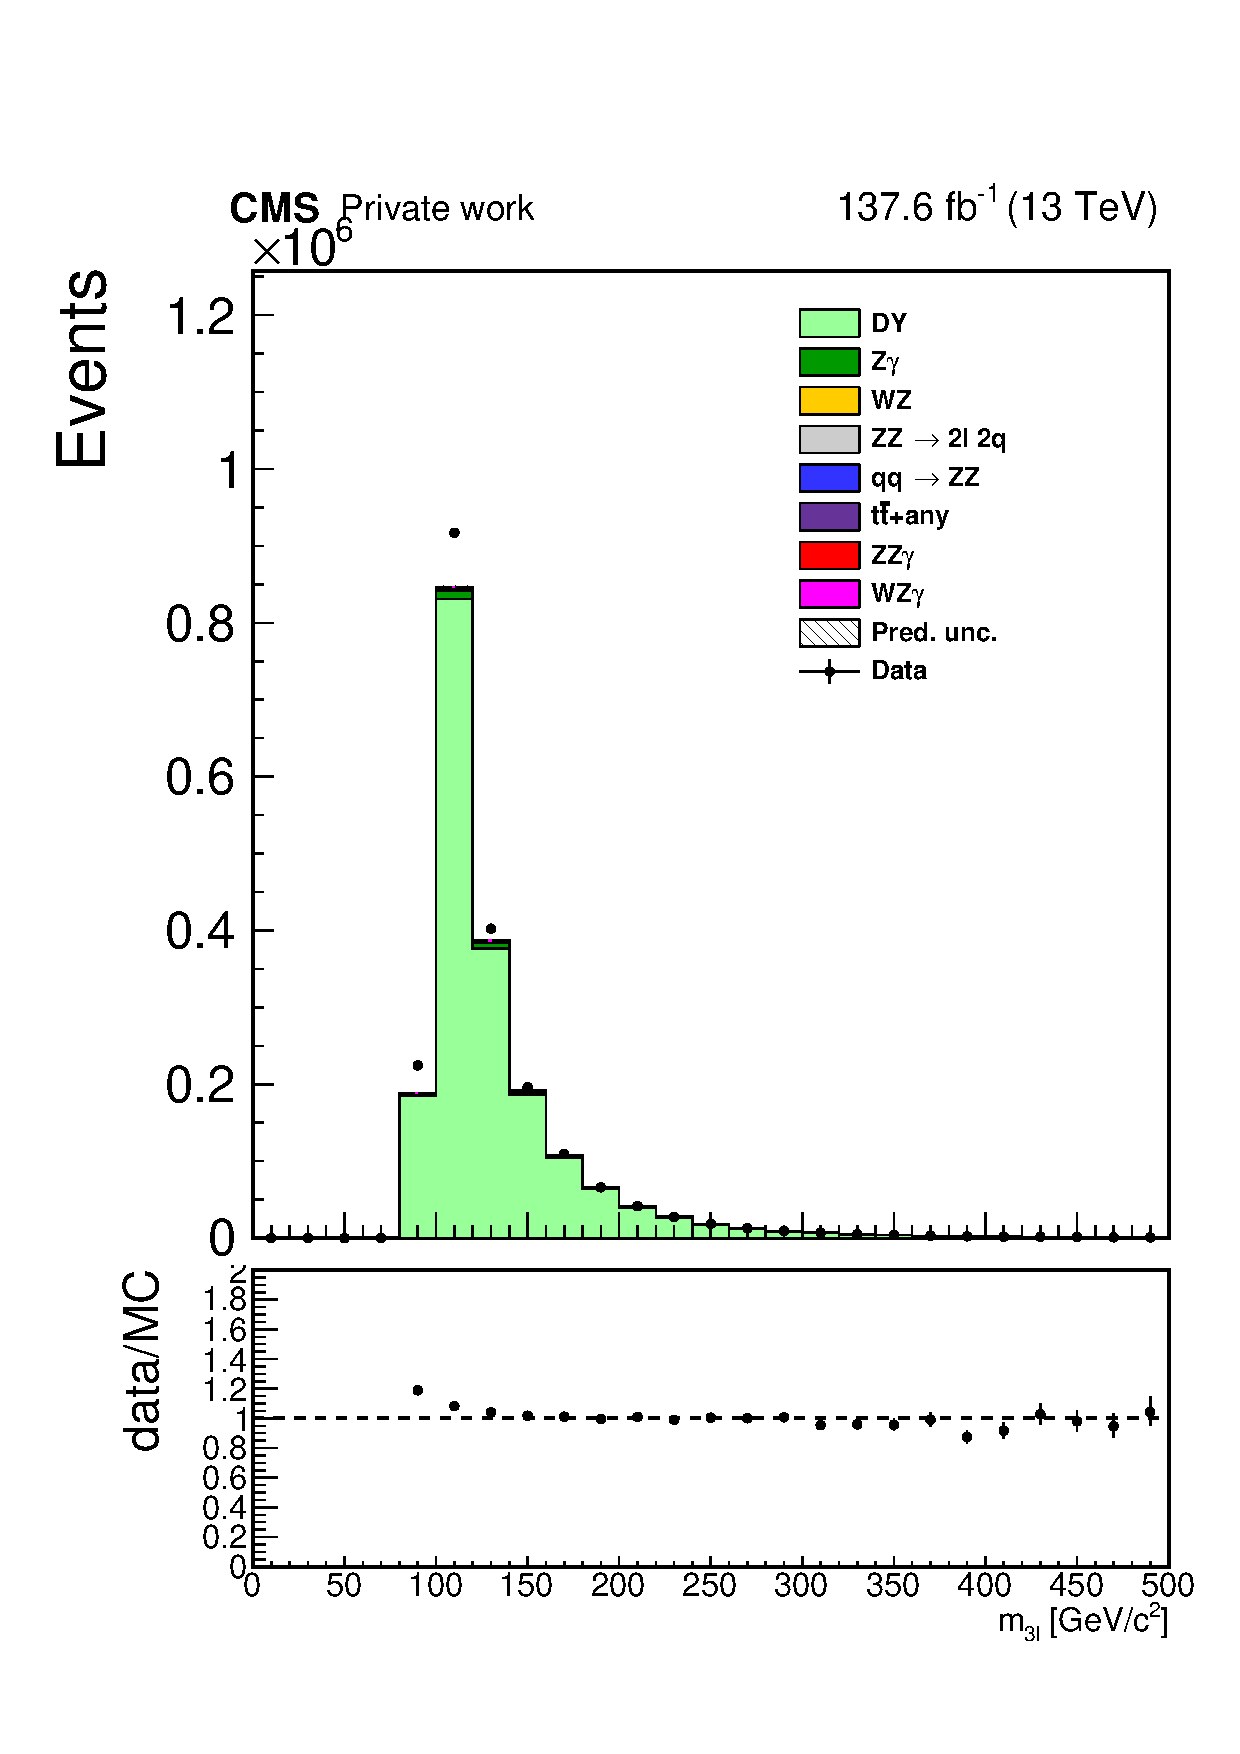
\includegraphics[width=.4\textwidth]{VVGammaAnalyzer/Run2/fullMC/CRLFR/ZL_mass_pow.pdf}}\quad
  \subfigure [] {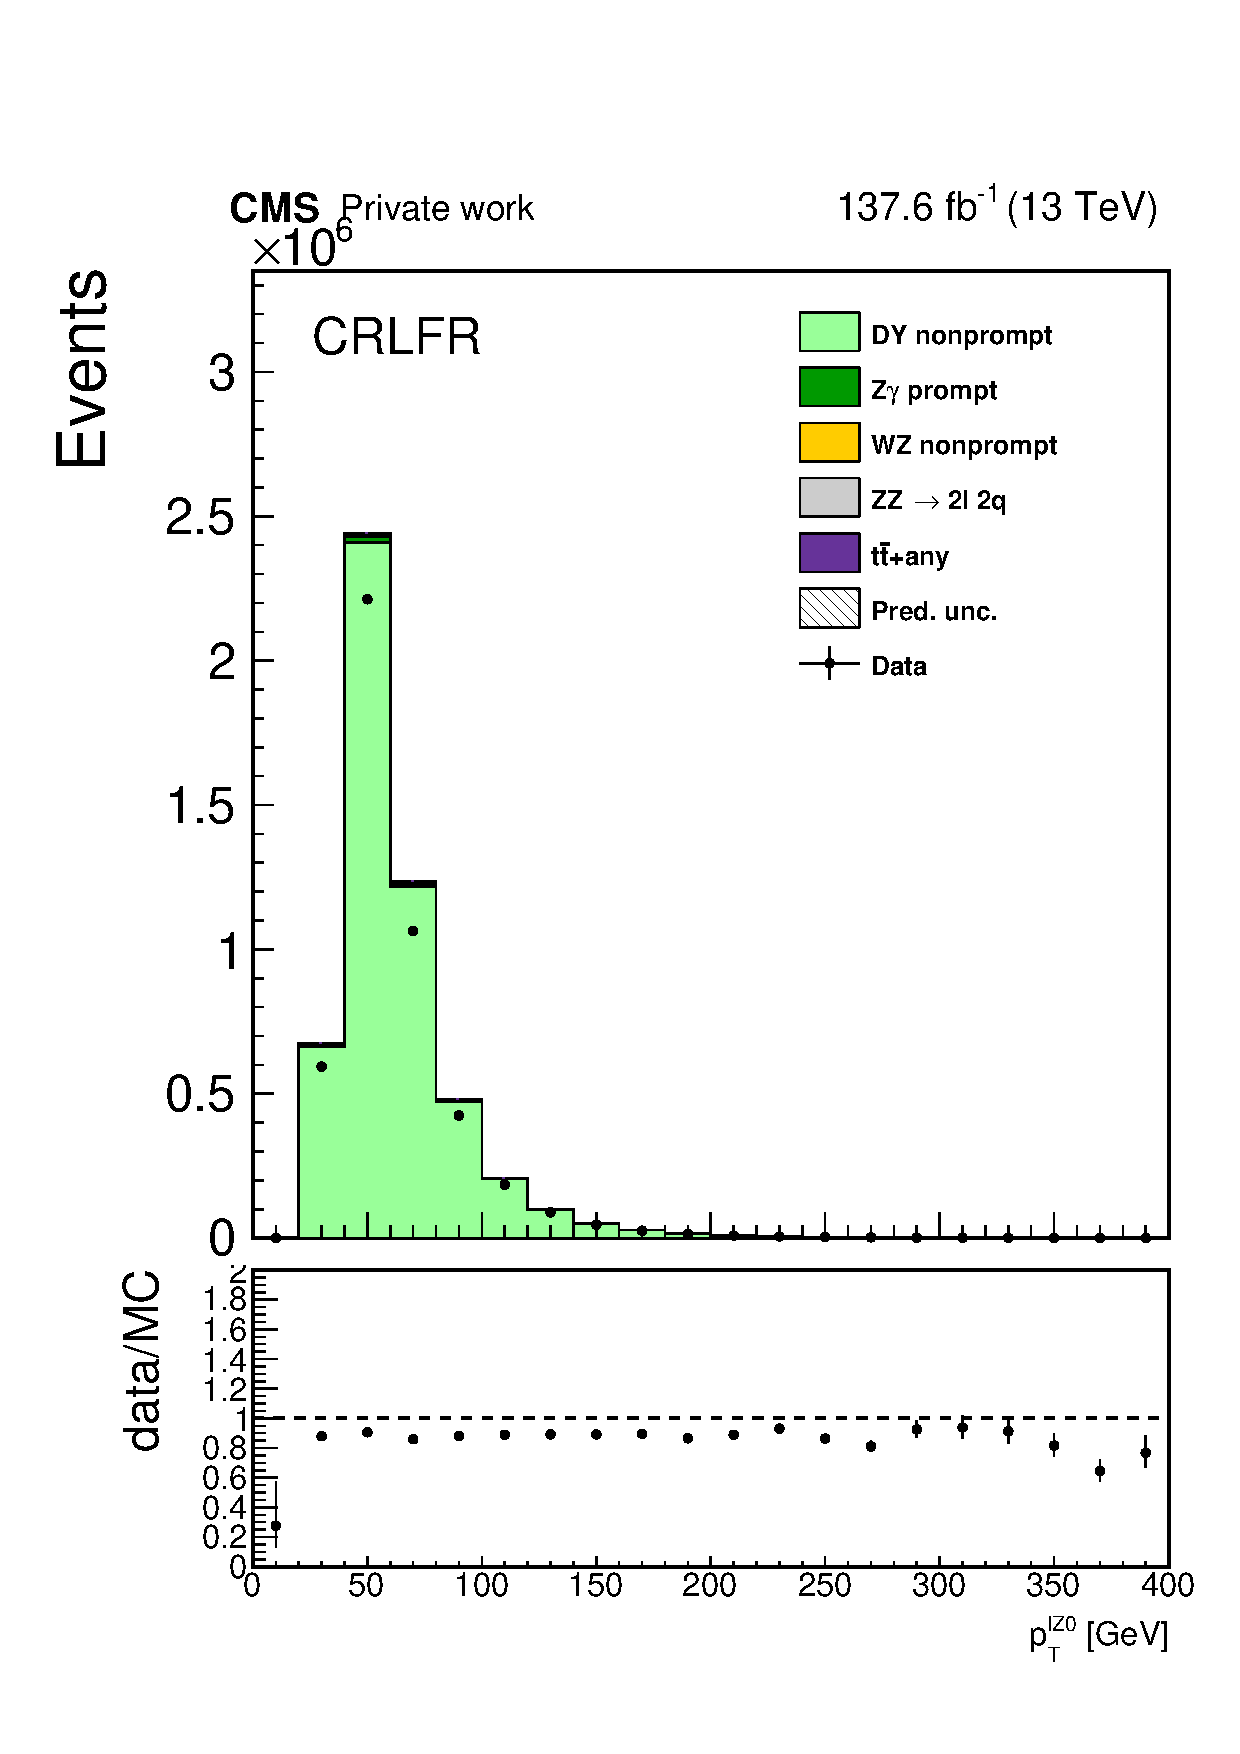
\includegraphics[width=.4\textwidth]{VVGammaAnalyzer/Run2/fullMC/CRLFR/Z_l0_pt_pow.pdf}}
  \caption{Invariant mass of the three lepton system and transverse momentum of the leading lepton from the Z candidate
  in the fake rate measurement region, integrated on the whole Run2 period.}
  \label{fig:CRLFR_inclusive}
\end{figure}

\begin{figure}
  \centering
  \subfigure [] {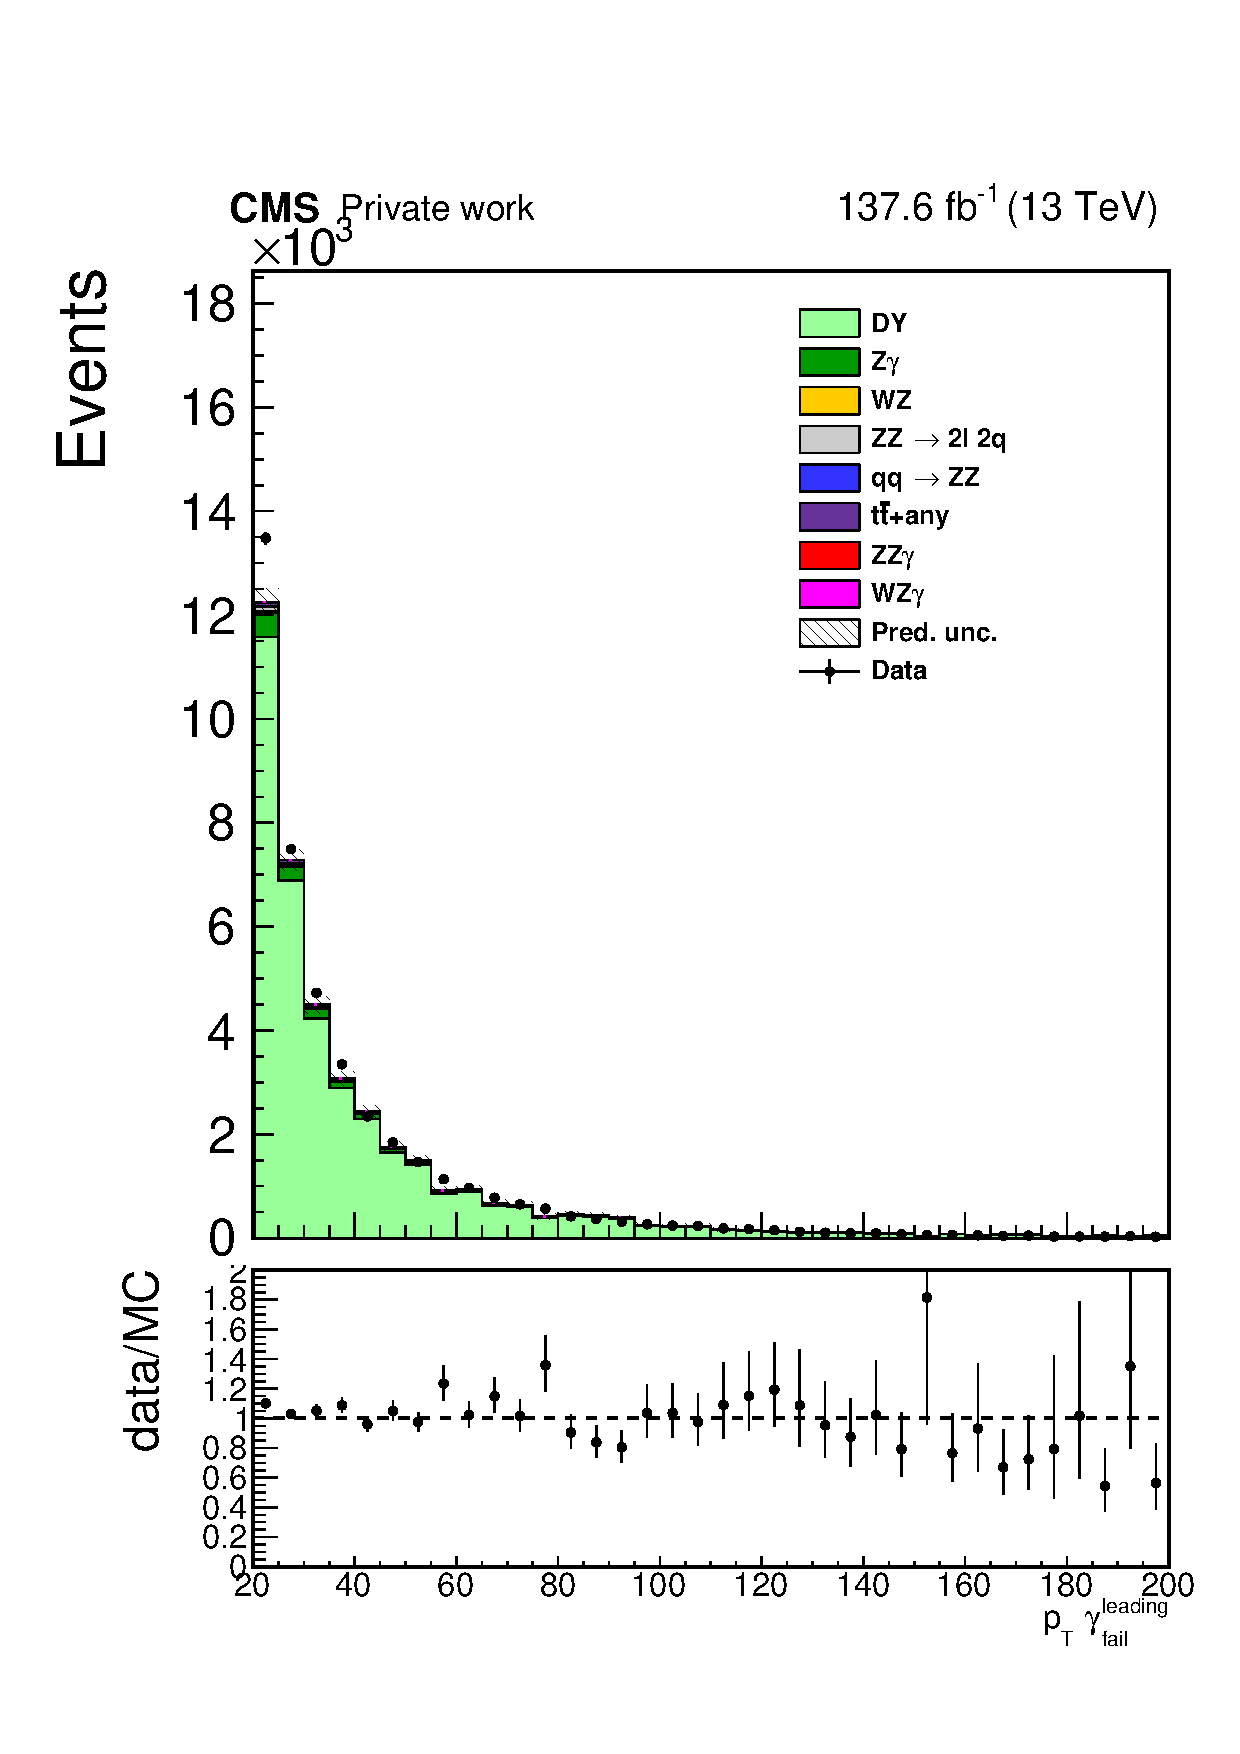
\includegraphics[width=.4\textwidth]{VVGammaAnalyzer/Run2/fullMC/CRLFR/lead_fail_pt_fine_pow.pdf}}\quad
  \subfigure [] {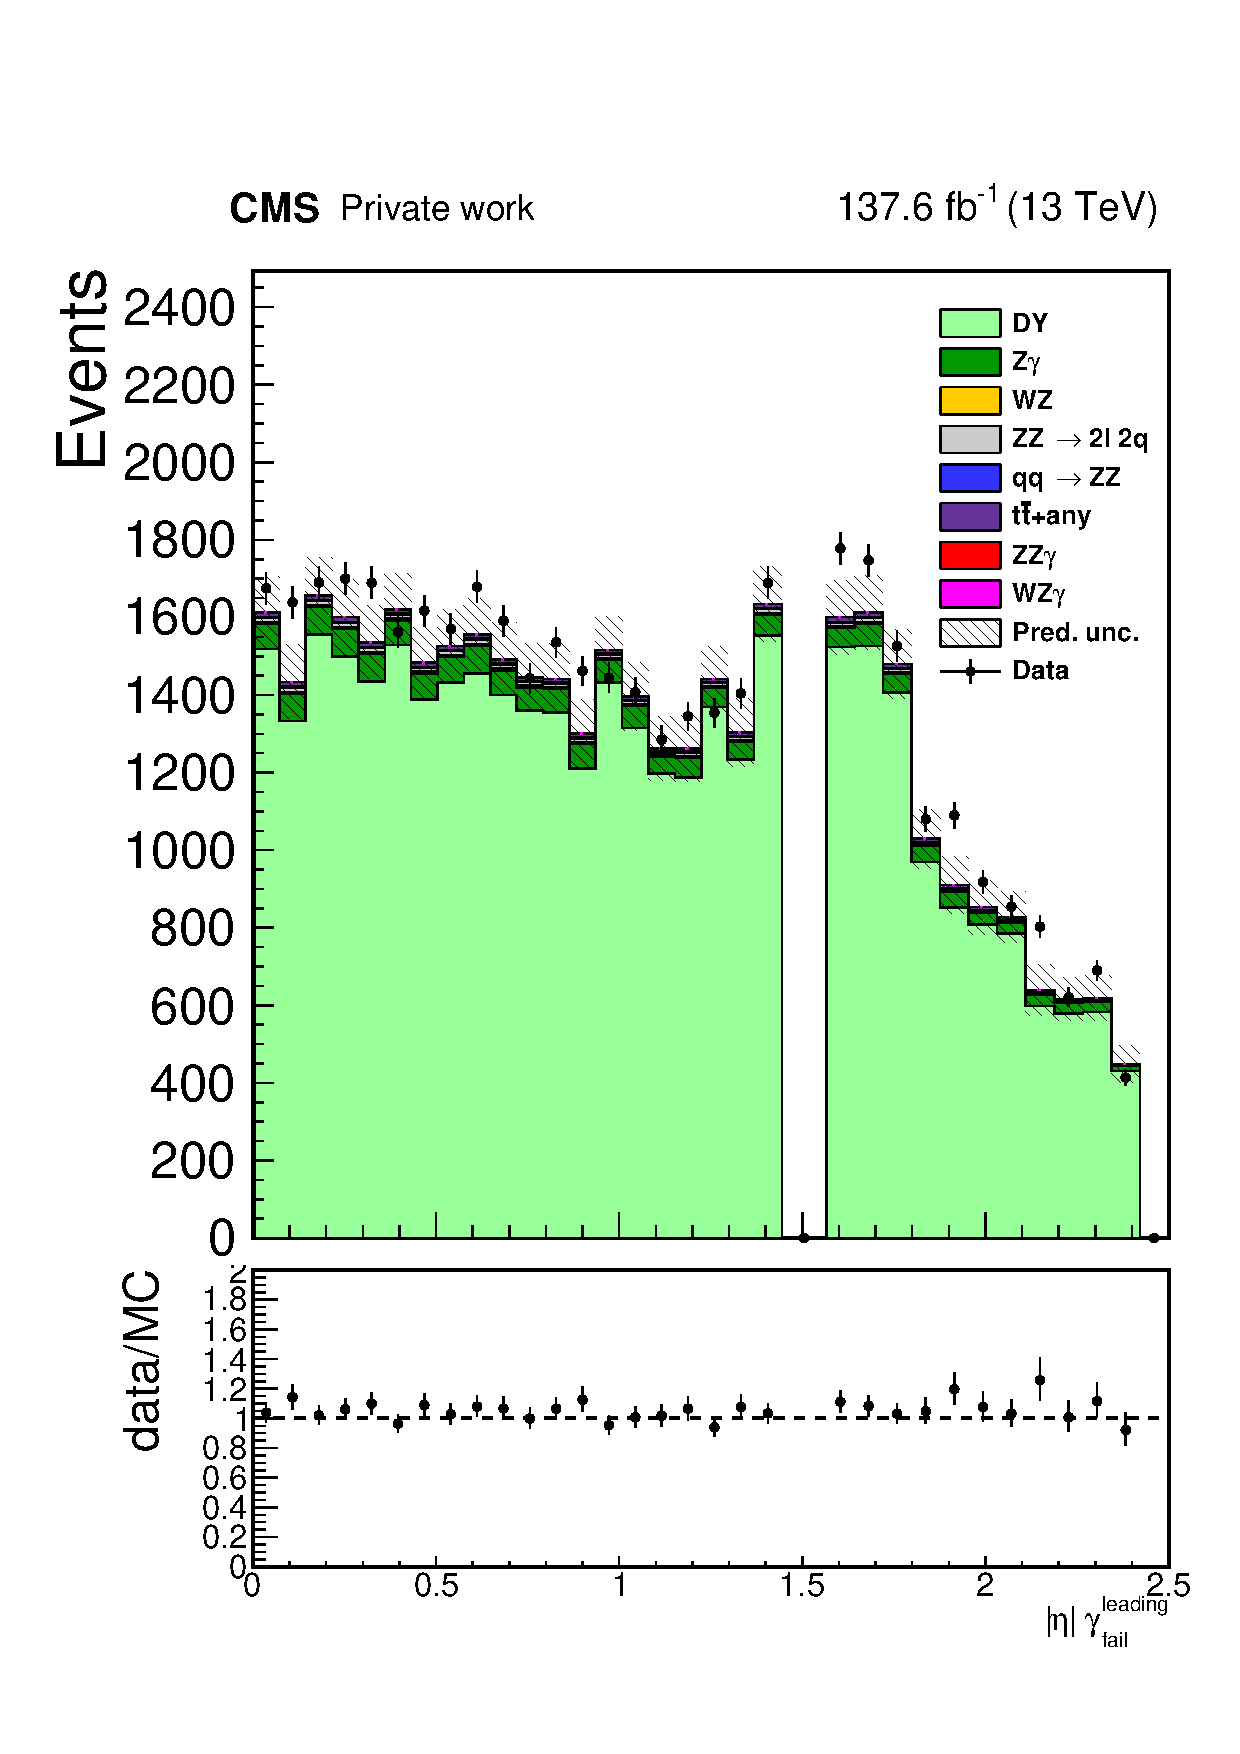
\includegraphics[width=.4\textwidth]{VVGammaAnalyzer/Run2/fullMC/CRLFR/lead_fail_aeta_fine_pow.pdf}}
  \caption{Transverse momentum and pseudorapidity of photons passing the loose criterion (VeryLoose ID) but failing the tight selection (Loose working point of the cut-based ID)
    in the fake rate measurement region, integrated on the whole Run2 period.}
  \label{fig:CRLFR_lead_fail}
\end{figure}

\begin{figure}
  \centering
  \subfigure [] {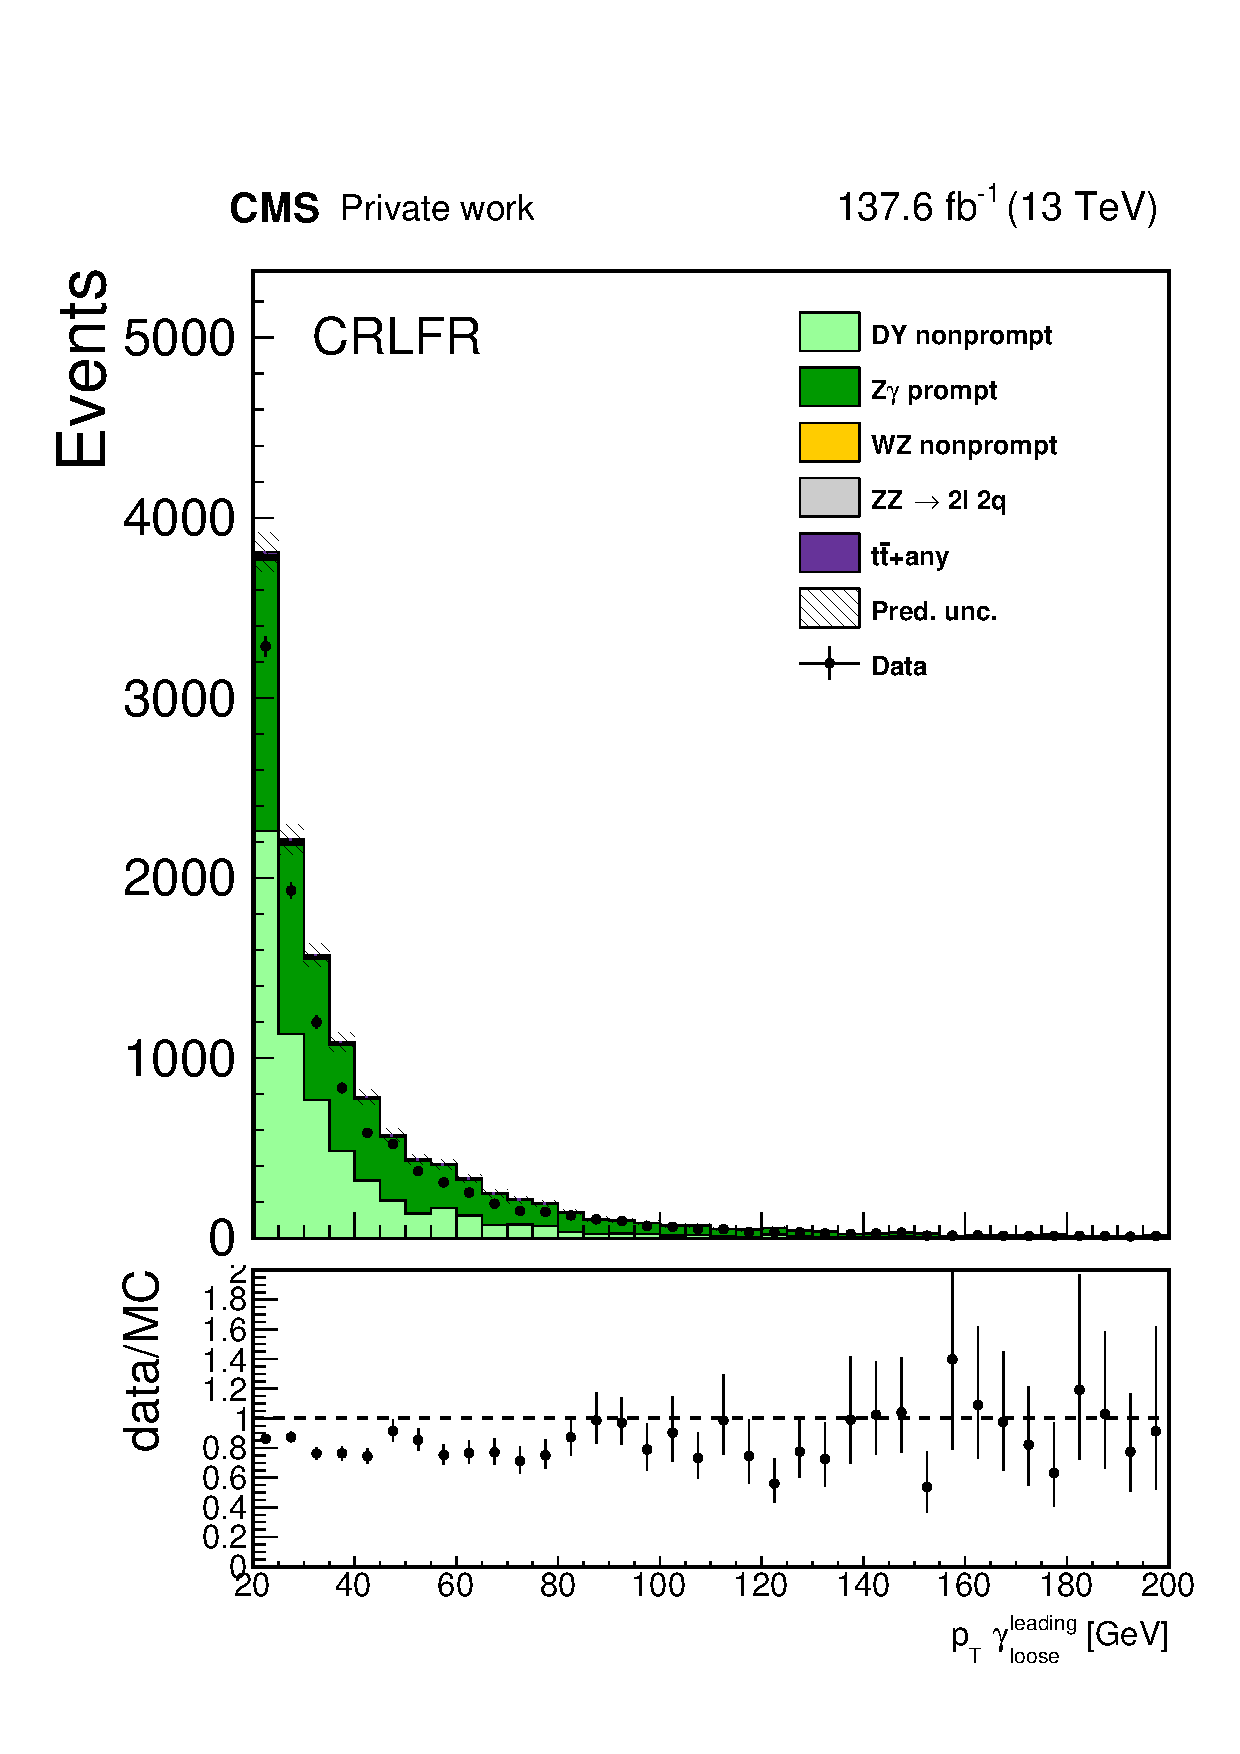
\includegraphics[width=.4\textwidth]{VVGammaAnalyzer/Run2/fullMC/CRLFR/lead_loose_pt_fine_pow.pdf}}\quad
  \subfigure [] {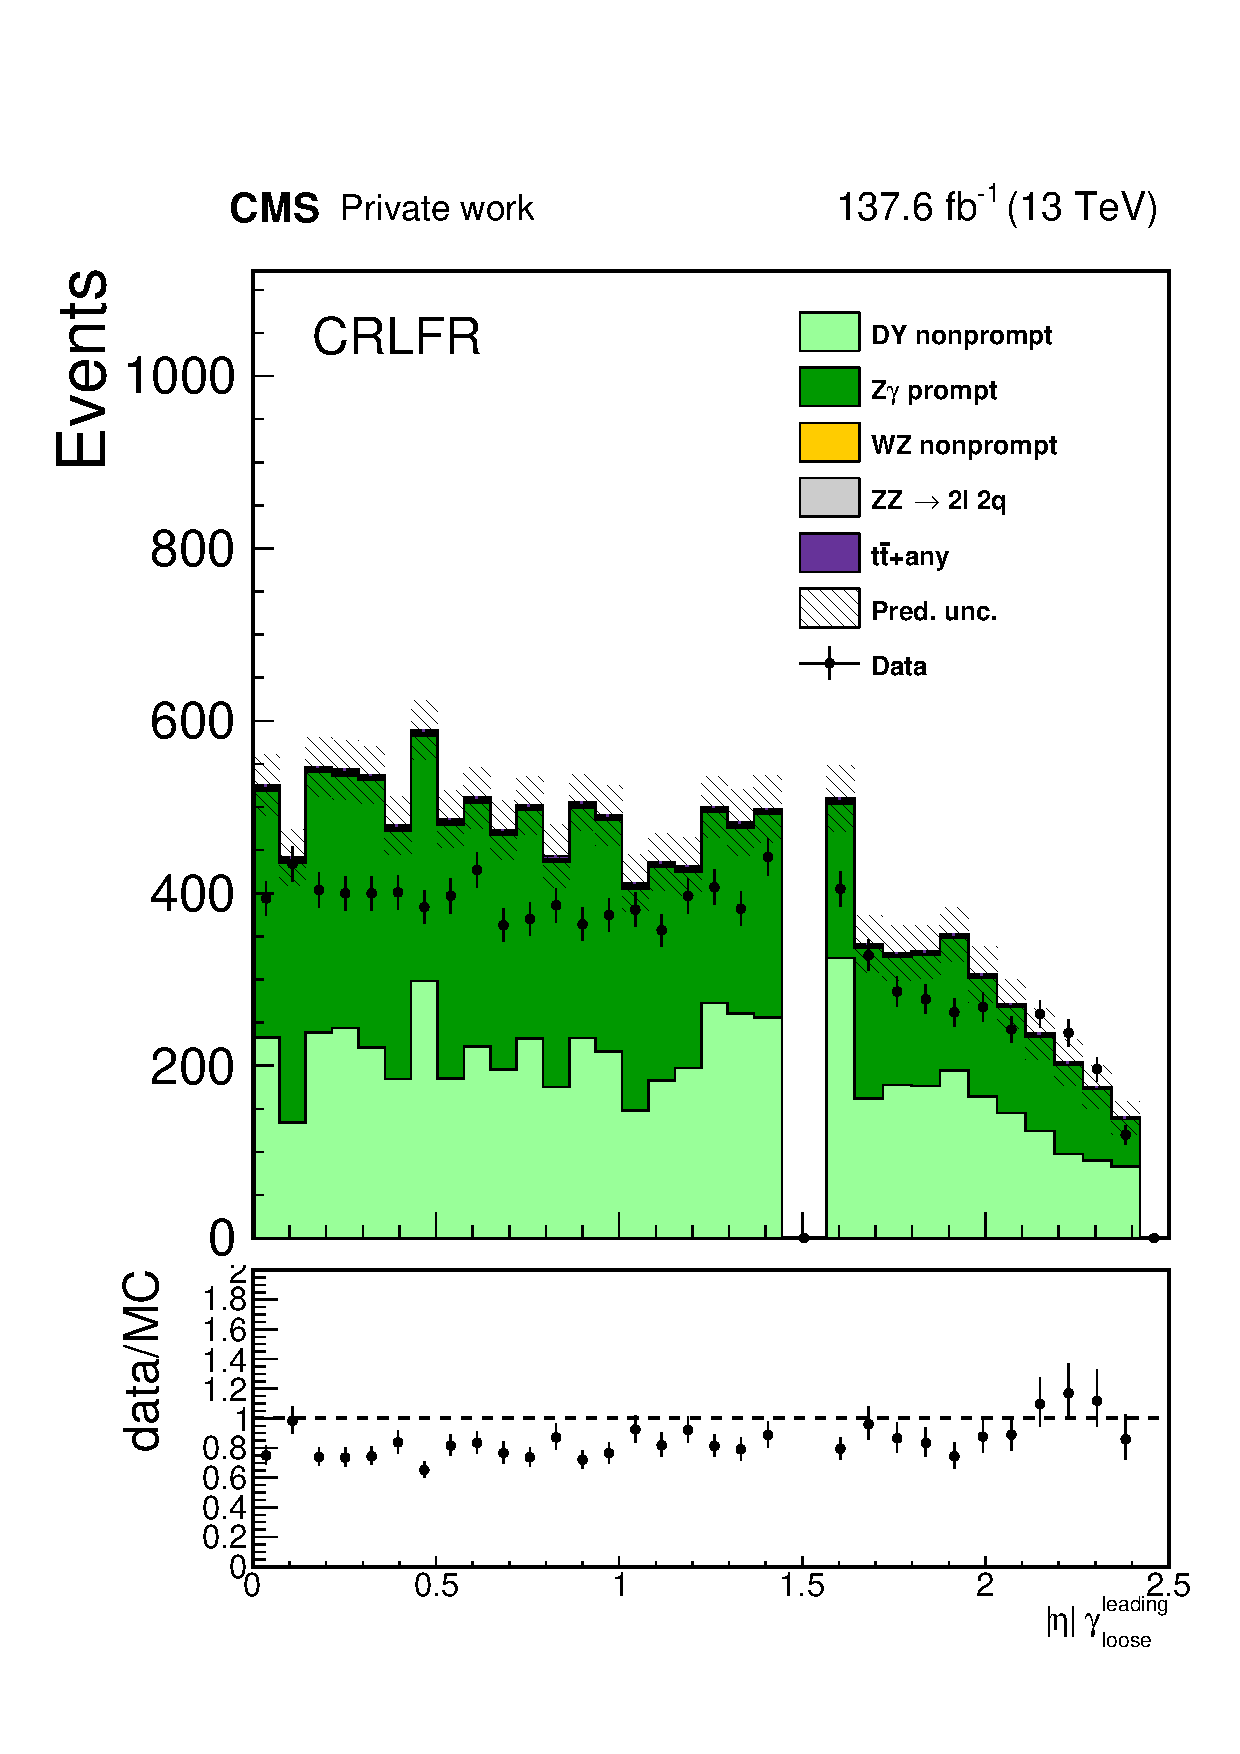
\includegraphics[width=.4\textwidth]{VVGammaAnalyzer/Run2/fullMC/CRLFR/lead_loose_aeta_fine_pow.pdf}}
  \caption{Transverse momentum and pseudorapidity of photons passing the tight selection (Loose working point of the cut-based ID)
    in the fake rate measurement region, integrated on the whole Run2 period.}
  \label{fig:CRLFR_lead_pass}
\end{figure}

The fake rate is then measured as the ratio of events in which the photon passes also the tight selection (the Loose working point of the cut-based ID)
to the total.
This measurement is done separately for endcap and barrel, for several bins of \pt (Figure \ref{fig:phFR_VLtoL}).

\begin{figure}
\subfigure [2016preVFP ] {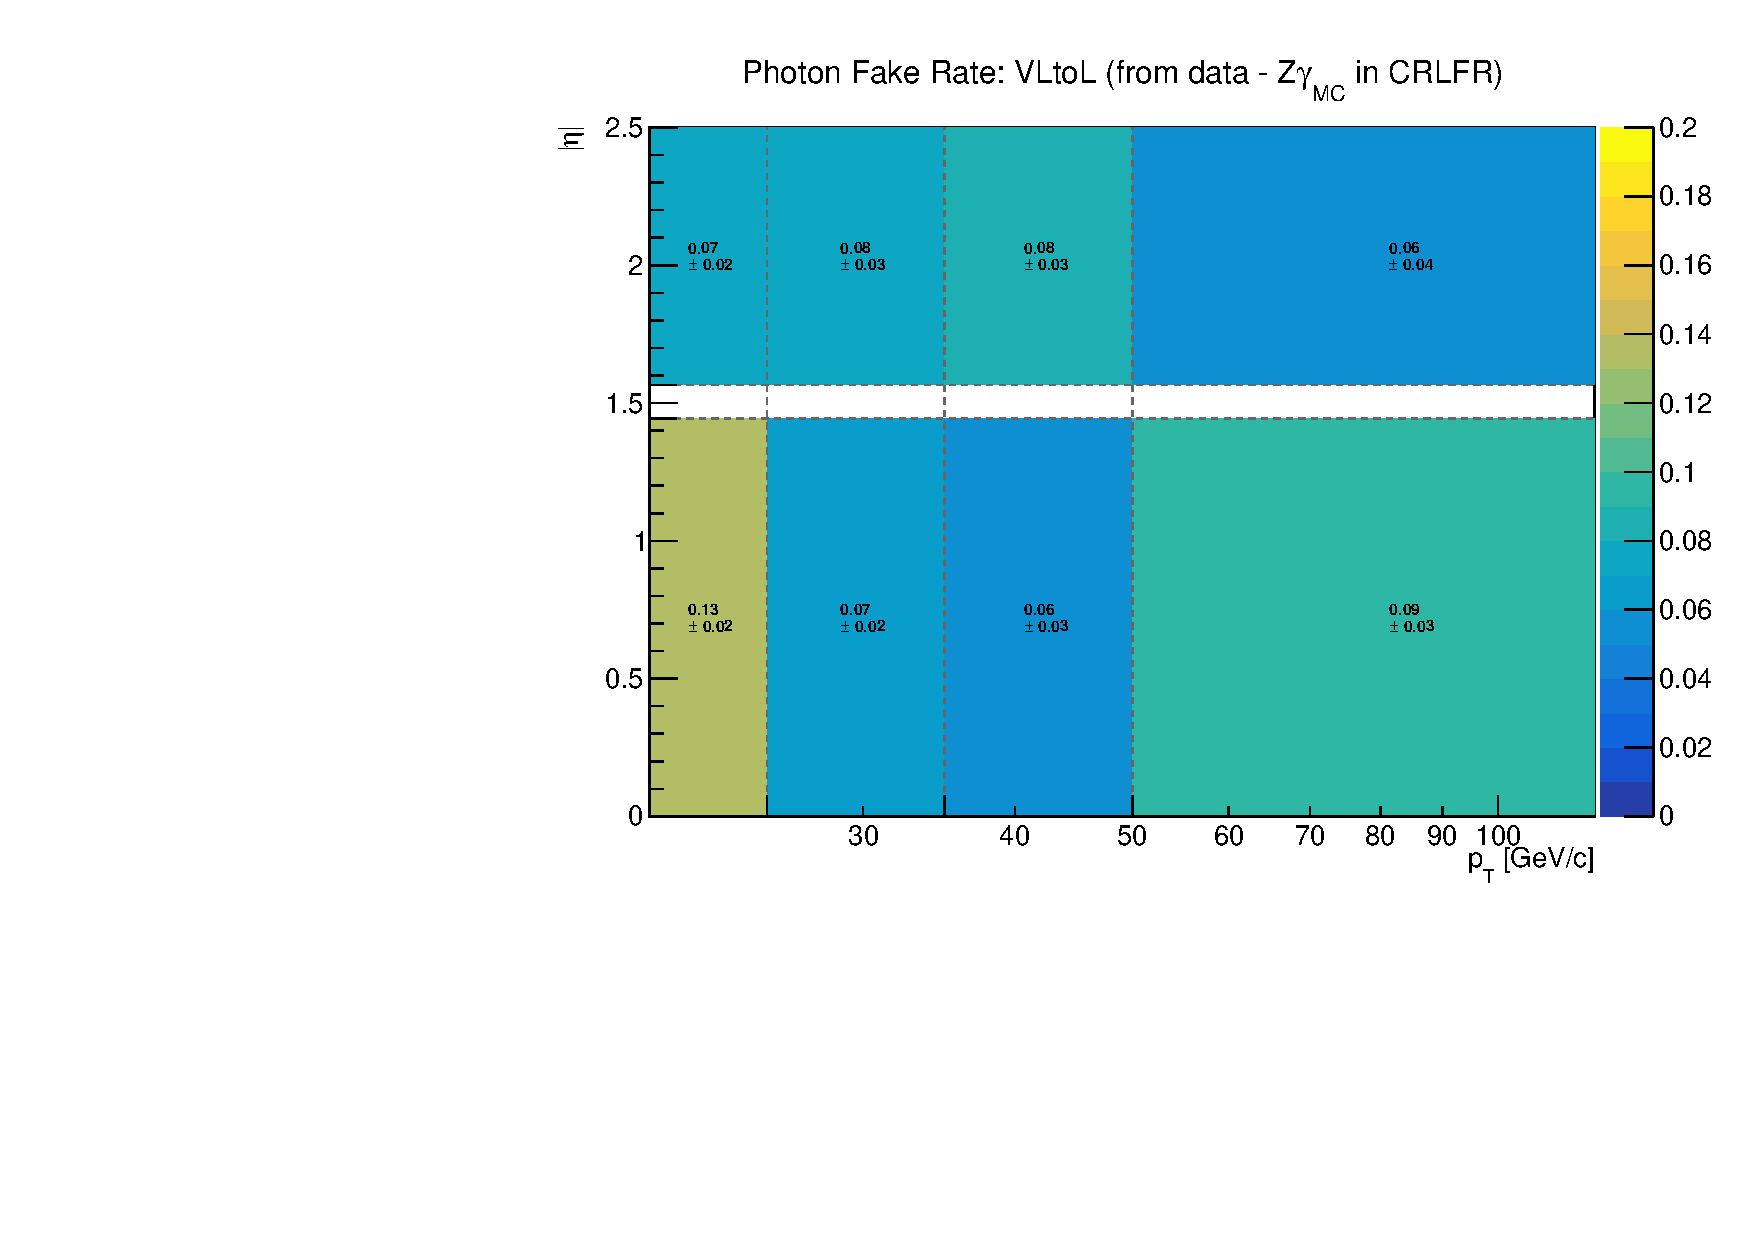
\includegraphics[width=.5\textwidth]{Figures/FR_VLtoL_pt-aeta_data-ZGToLLG_2016preVFP.pdf}}%
\subfigure [2016postVFP] {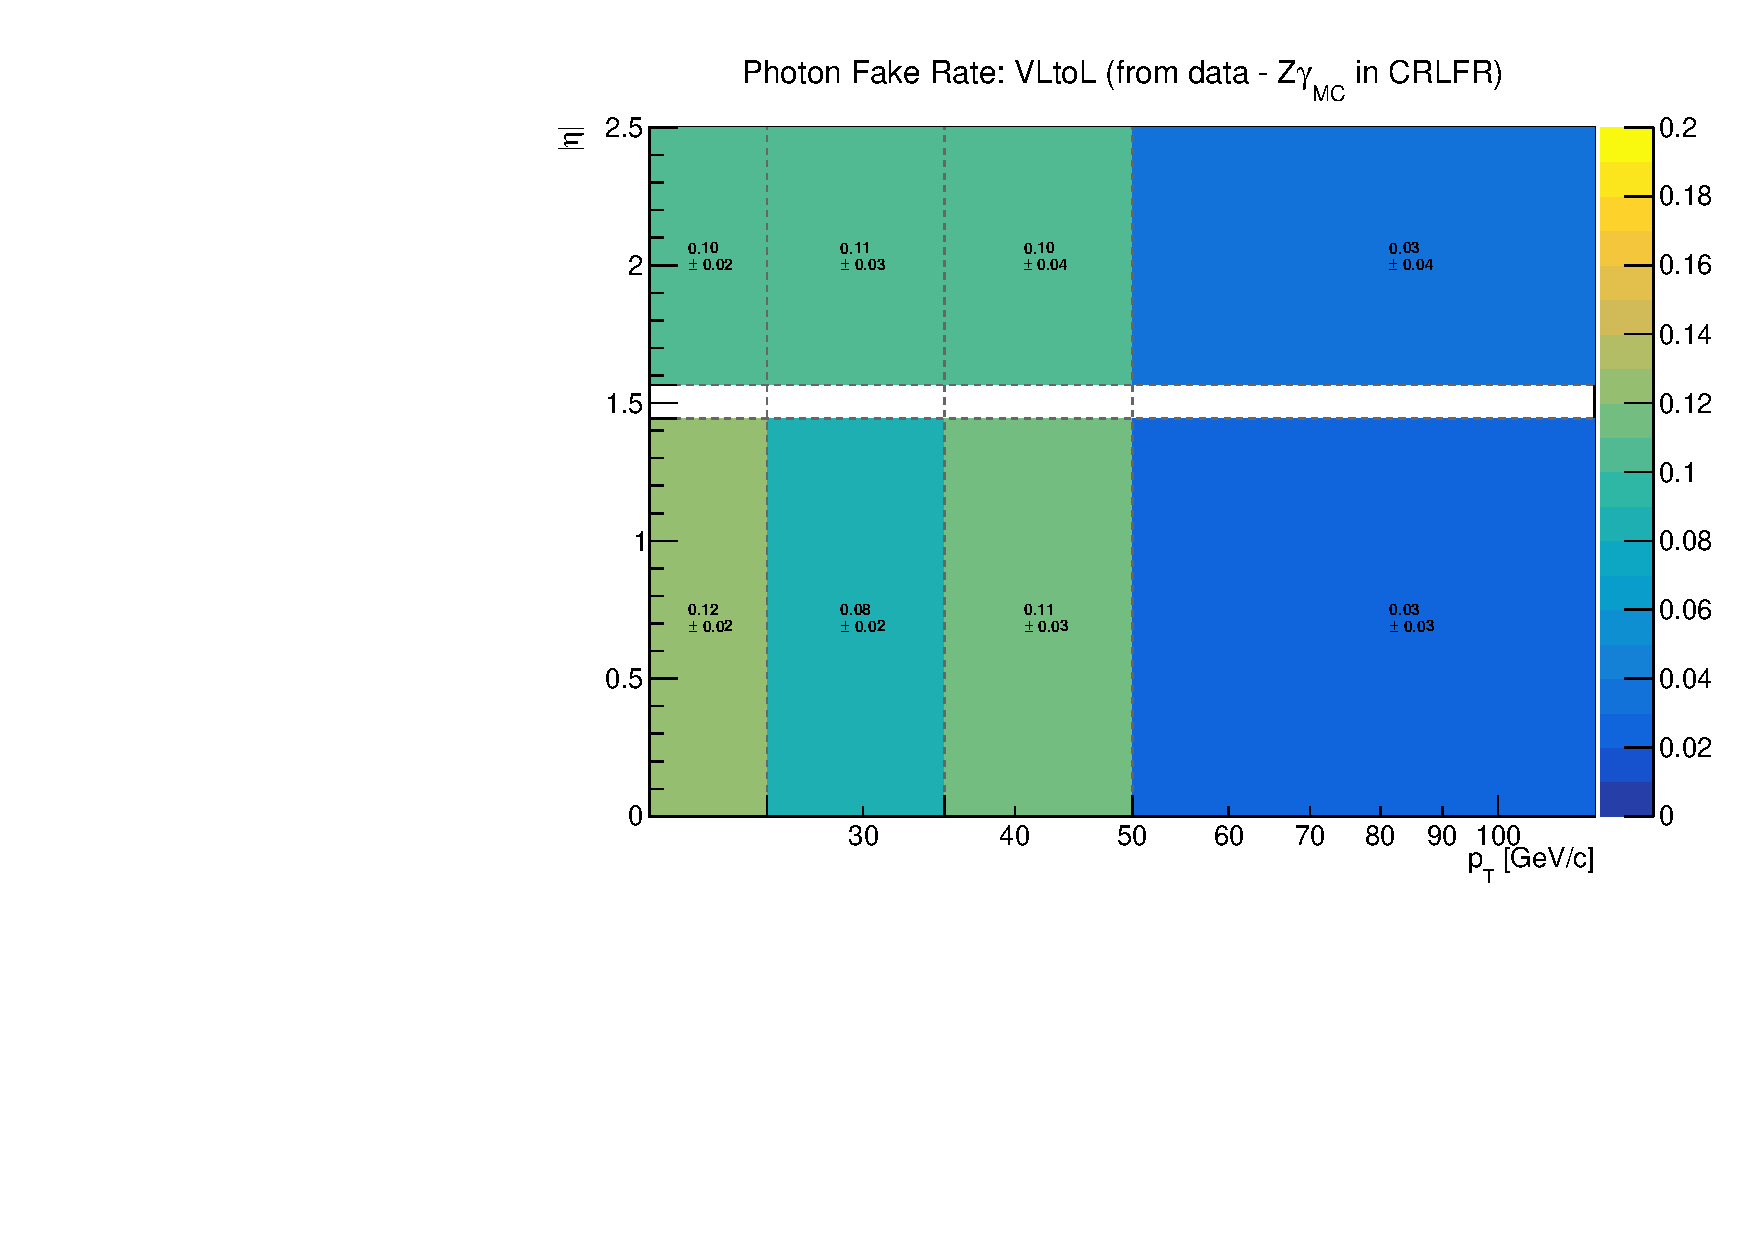
\includegraphics[width=.5\textwidth]{Figures/FR_VLtoL_pt-aeta_data-ZGToLLG_2016postVFP.pdf}}\\
\subfigure [2017]        {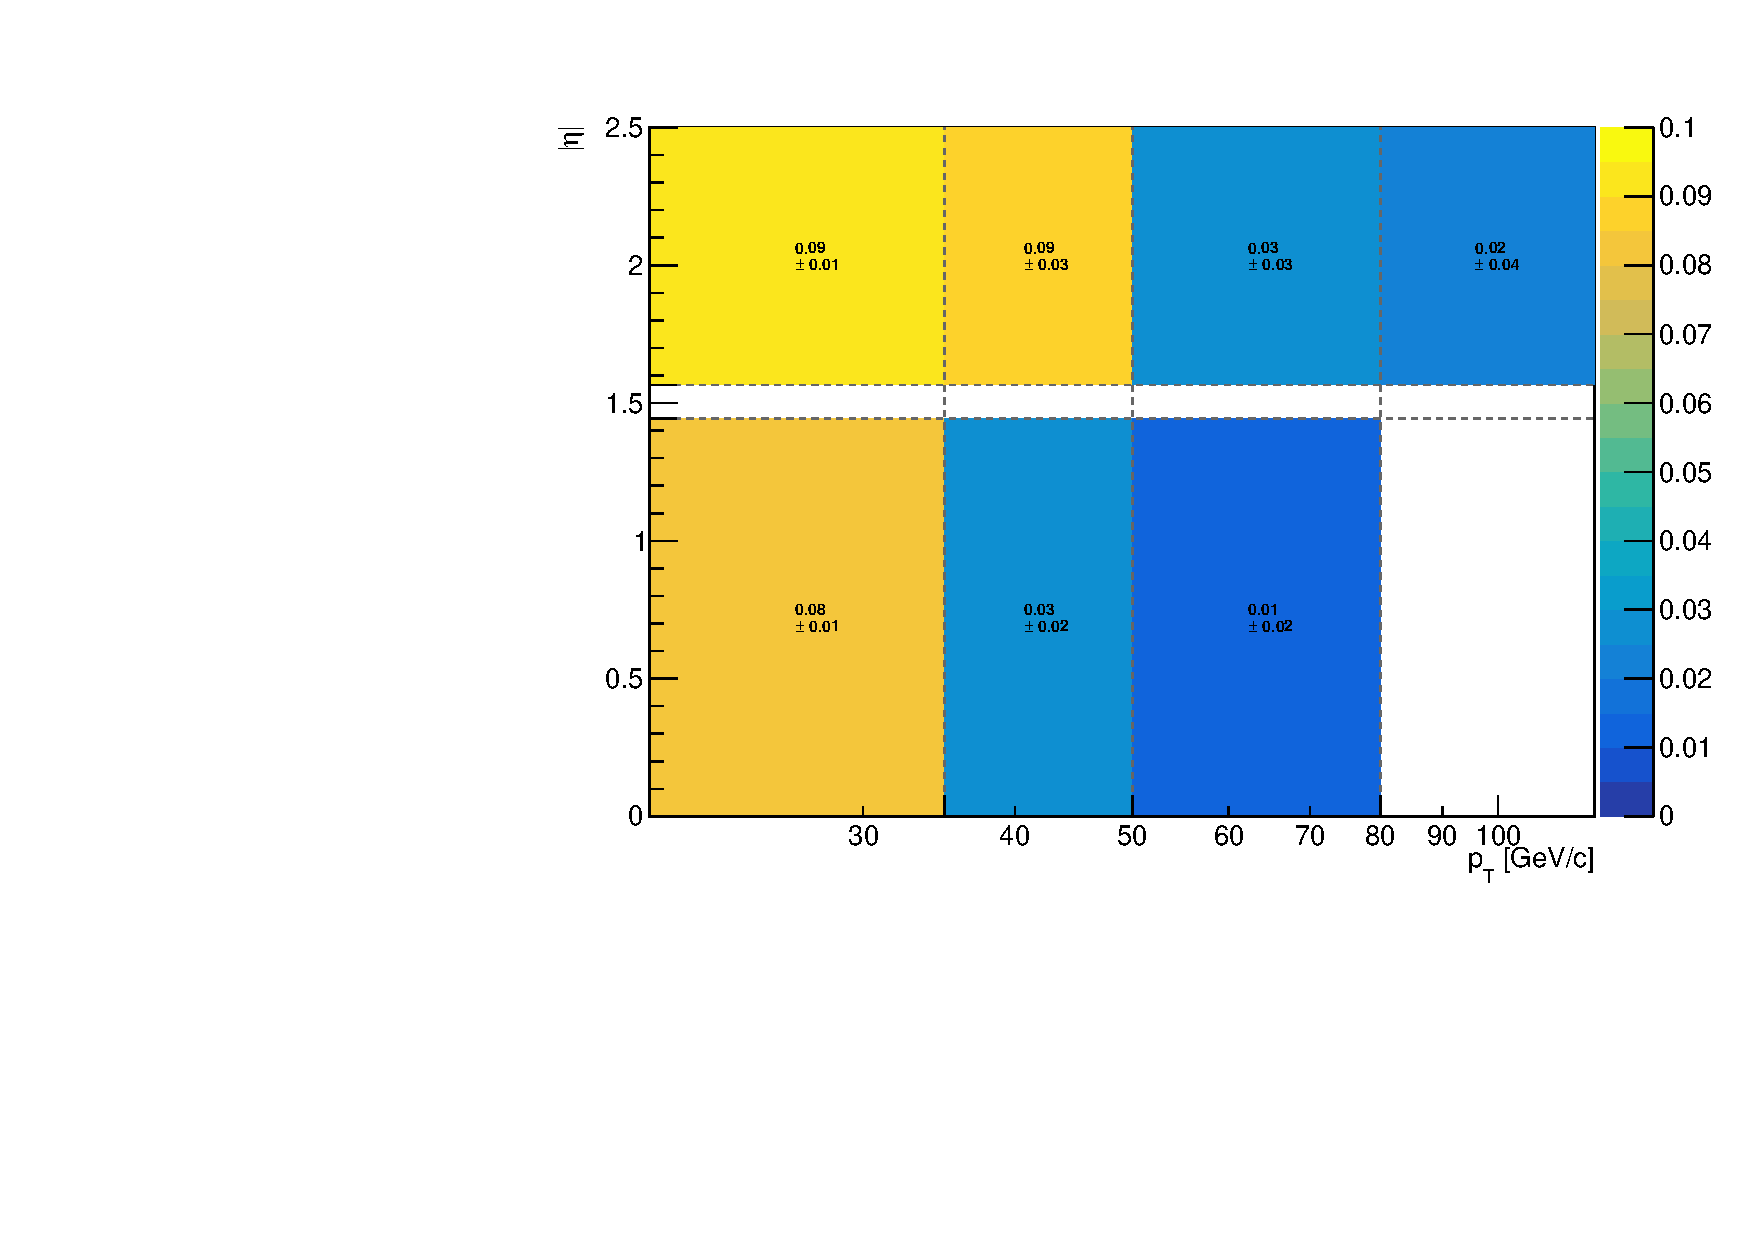
\includegraphics[width=.5\textwidth]{Figures/FR_VLtoL_pt-aeta_data-ZGToLLG_2017.pdf}}%
\subfigure [2018]        {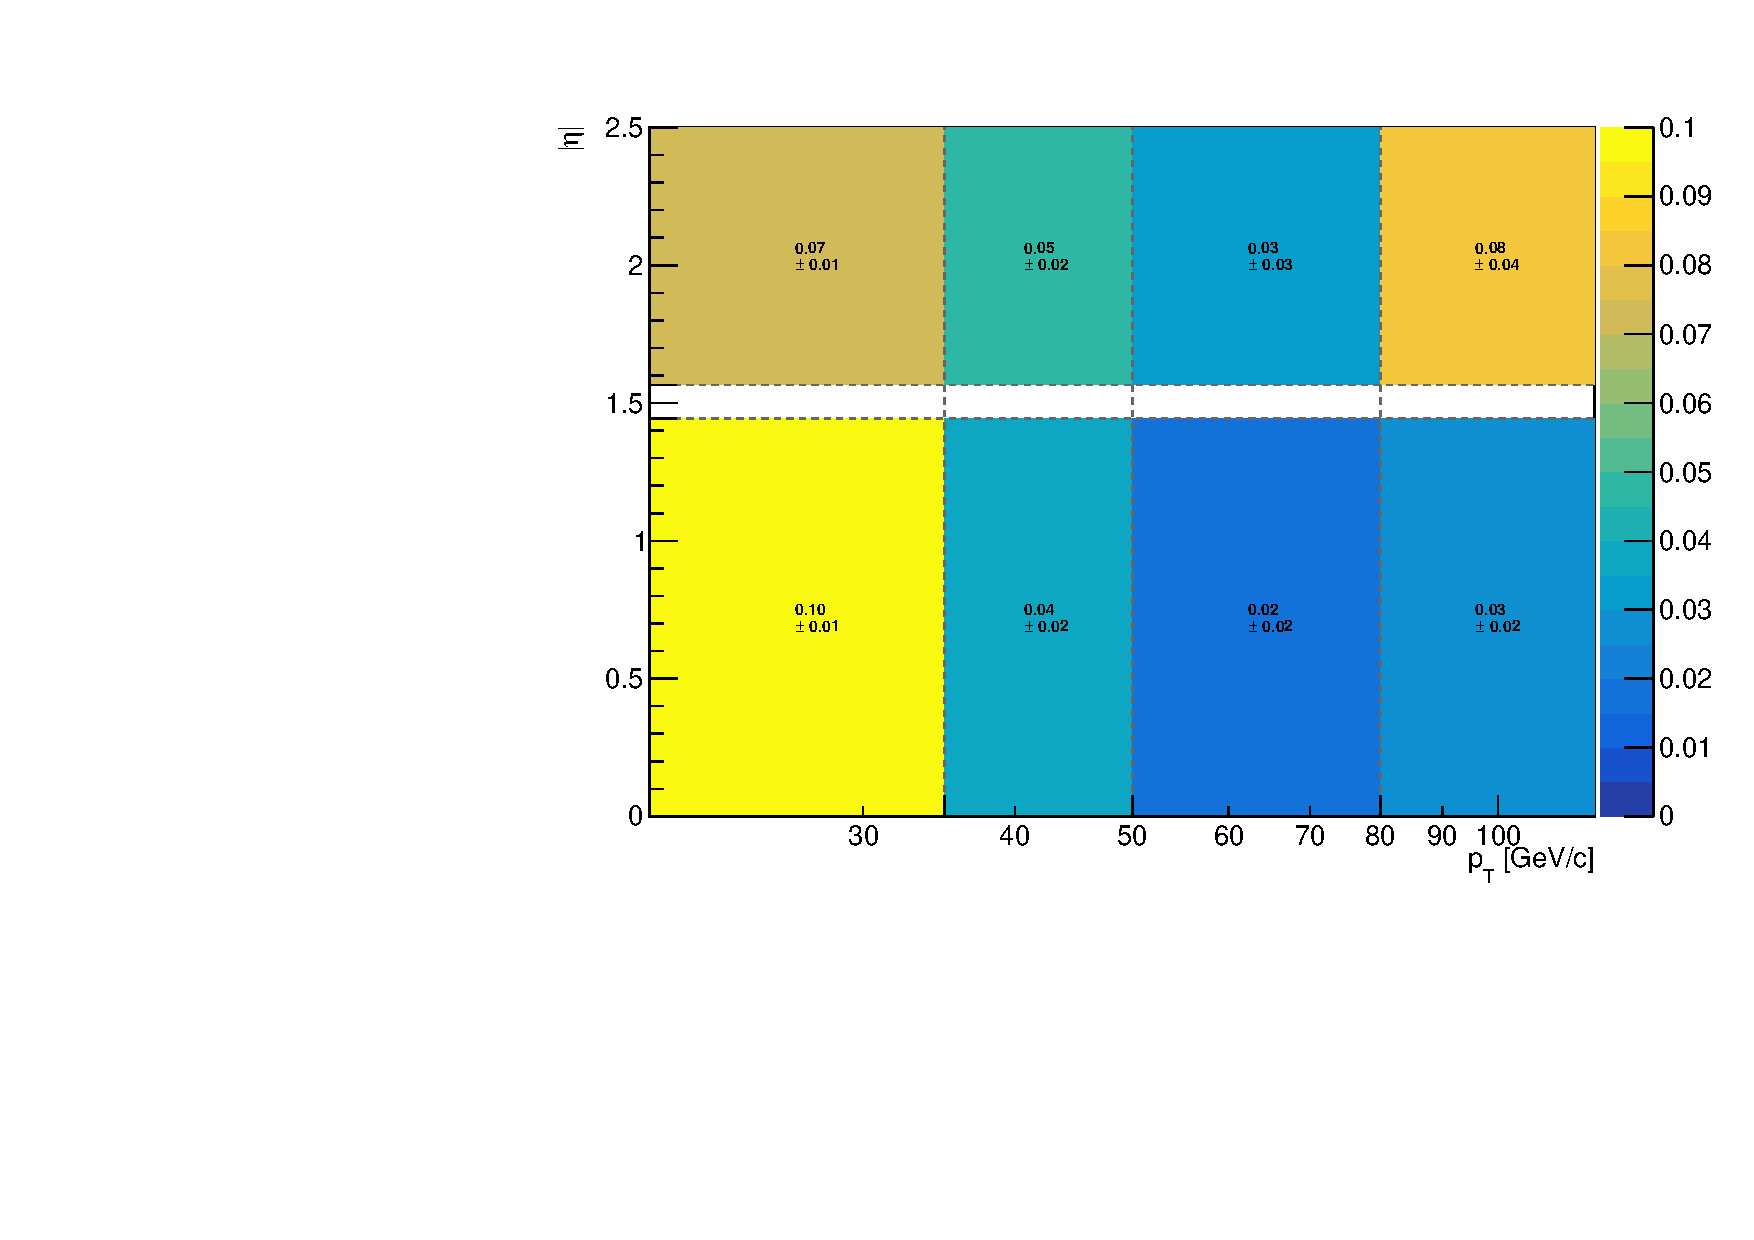
\includegraphics[width=.5\textwidth]{Figures/FR_VLtoL_pt-aeta_data-ZGToLLG_2018.pdf}}
\caption{Photon non-prompt rate as measured in data (with prompt $Z\gamma$ subtraction) using the cut-based ID for the photon.}
\label{fig:phFR_VLtoL}
\end{figure}

To ensure the stability of the measurement against other variables in the event,
additional measurements are carried out in specific sub-regions, and the results compared.
In particular, the effect of:
\begin{itemize}
\item The status of the third lepton: whether it passes or fails the tight selection.
  This could bias the measurement if the lepton were a misidentified jet and the additional hadronic activity produced an additional \nonprompt photon.
\item The flavour of the third lepton
\item The flavour of the SFOS pair that constitute the \PZ boson.
\item The number of additional jets in the event
\item The distance from the closest jet in the event
\end{itemize}

\note{Move to appendix? --> ``The results of these cross checks are in Appendix...''}

The photon non-prompt rate is assumed to be independent of the flavour of the leptons in the event.
This assumption is tested by deriving it separately for each flavour of the leptons of the Z boson $e^+ e^- \ell^\pm$ and $\mu^+ \mu^- \ell^\pm$, as shown in Figure \ref{fig:phFR_2e2m}.

\begin{figure}
\subfigure [$e^+ e^- \ell^\pm$]     {\resizebox{.5\textwidth}{!}{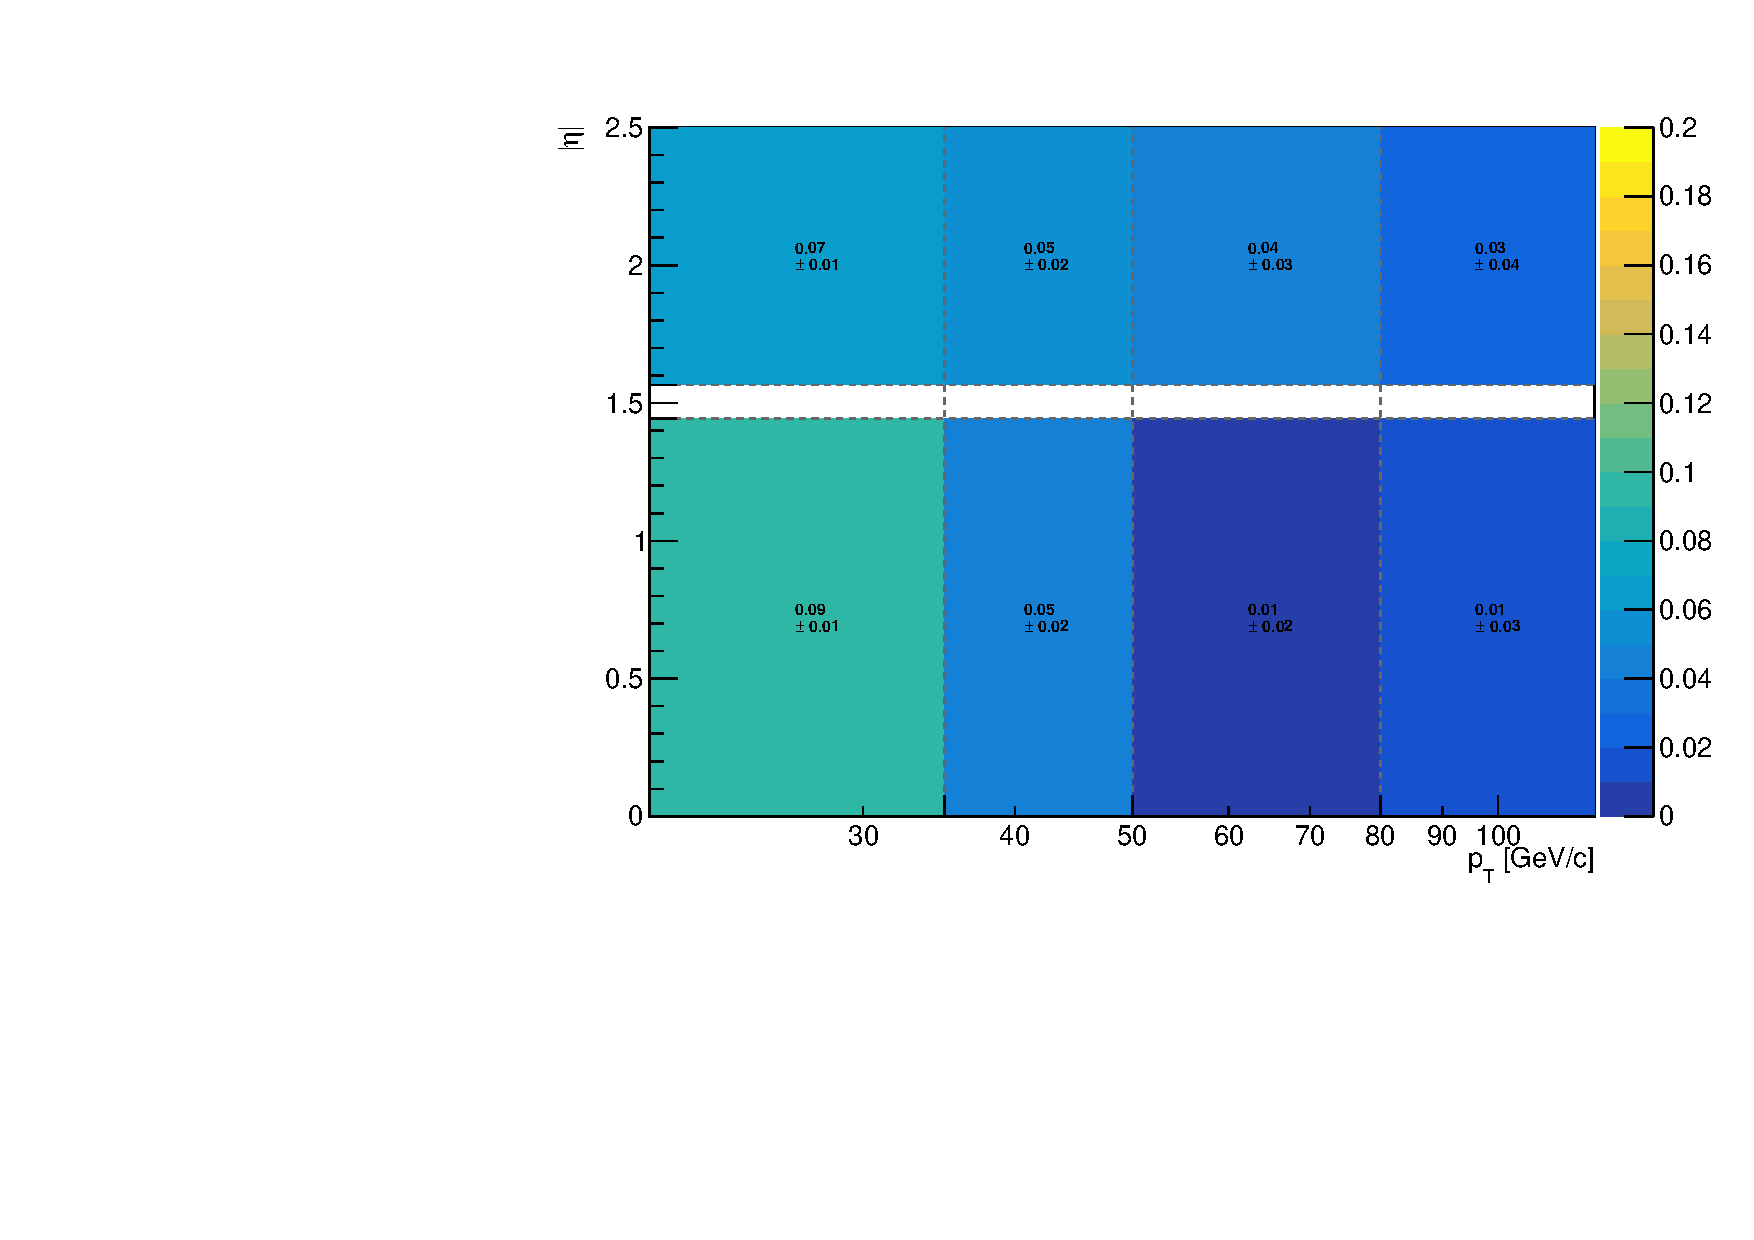
\includegraphics[width=.5\textwidth]{Figures/FR_VLtoL_pt-aeta_2e+x_data-ZGToLLG_2018.pdf}}}
\subfigure [$\mu^+ \mu^- \ell^\pm$] {\resizebox{.5\textwidth}{!}{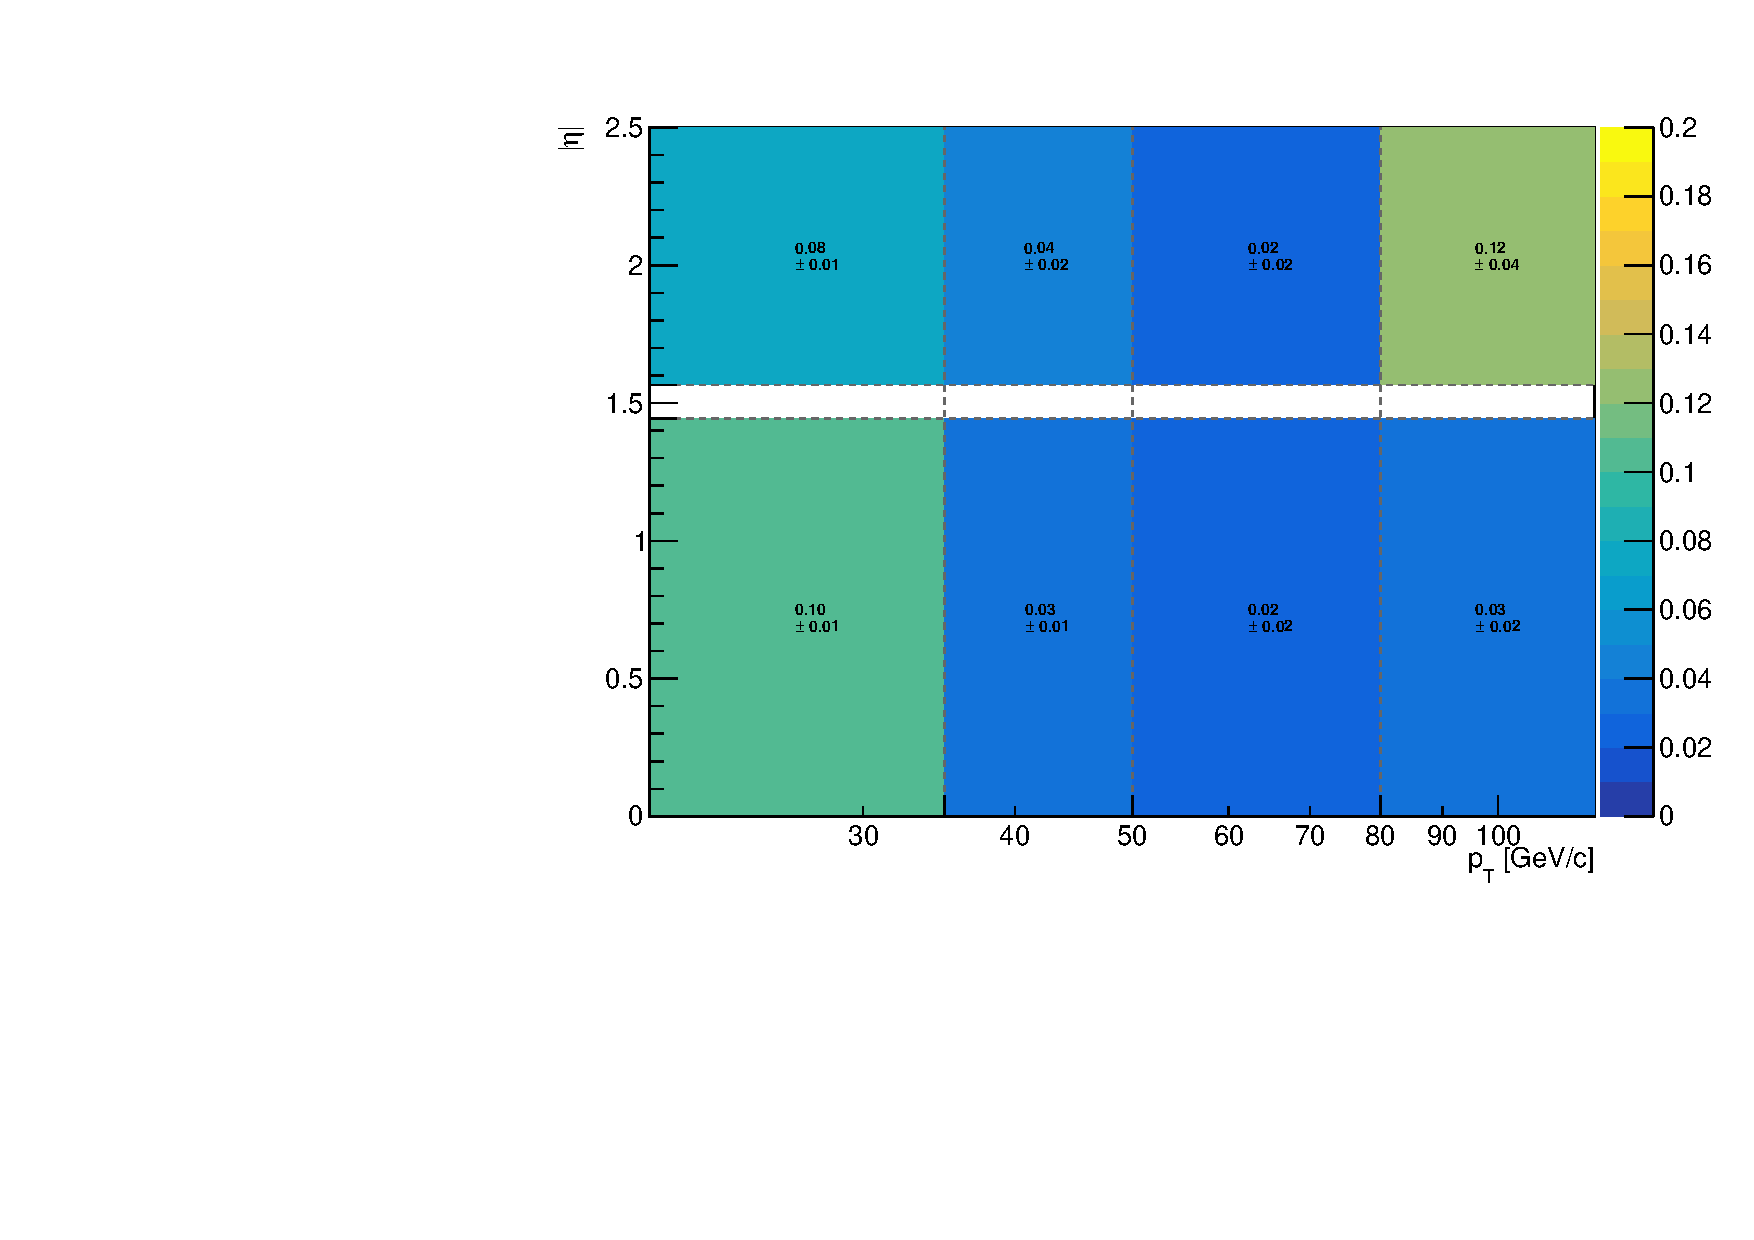
\includegraphics[width=.5\textwidth]{Figures/FR_VLtoL_pt-aeta_2m+x_data-ZGToLLG_2018.pdf}}}
\caption{Photon non-prompt rate as measured in 2018 data (with prompt $Z\gamma$ subtraction) in events with different lepton flavours for the Z boson.}
\label{fig:phFR_2e2m}
\end{figure}

The test is repeated for different flavours of the third lepton $\ell^+ \ell^- e^\pm$ and $\ell^+ \ell^- \mu^\pm$, and is shown in Figure \ref{fig:phFR_em}.

\begin{figure}
\subfigure [$\ell^+ \ell^- e^\pm$]   {\resizebox{.5\textwidth}{!}{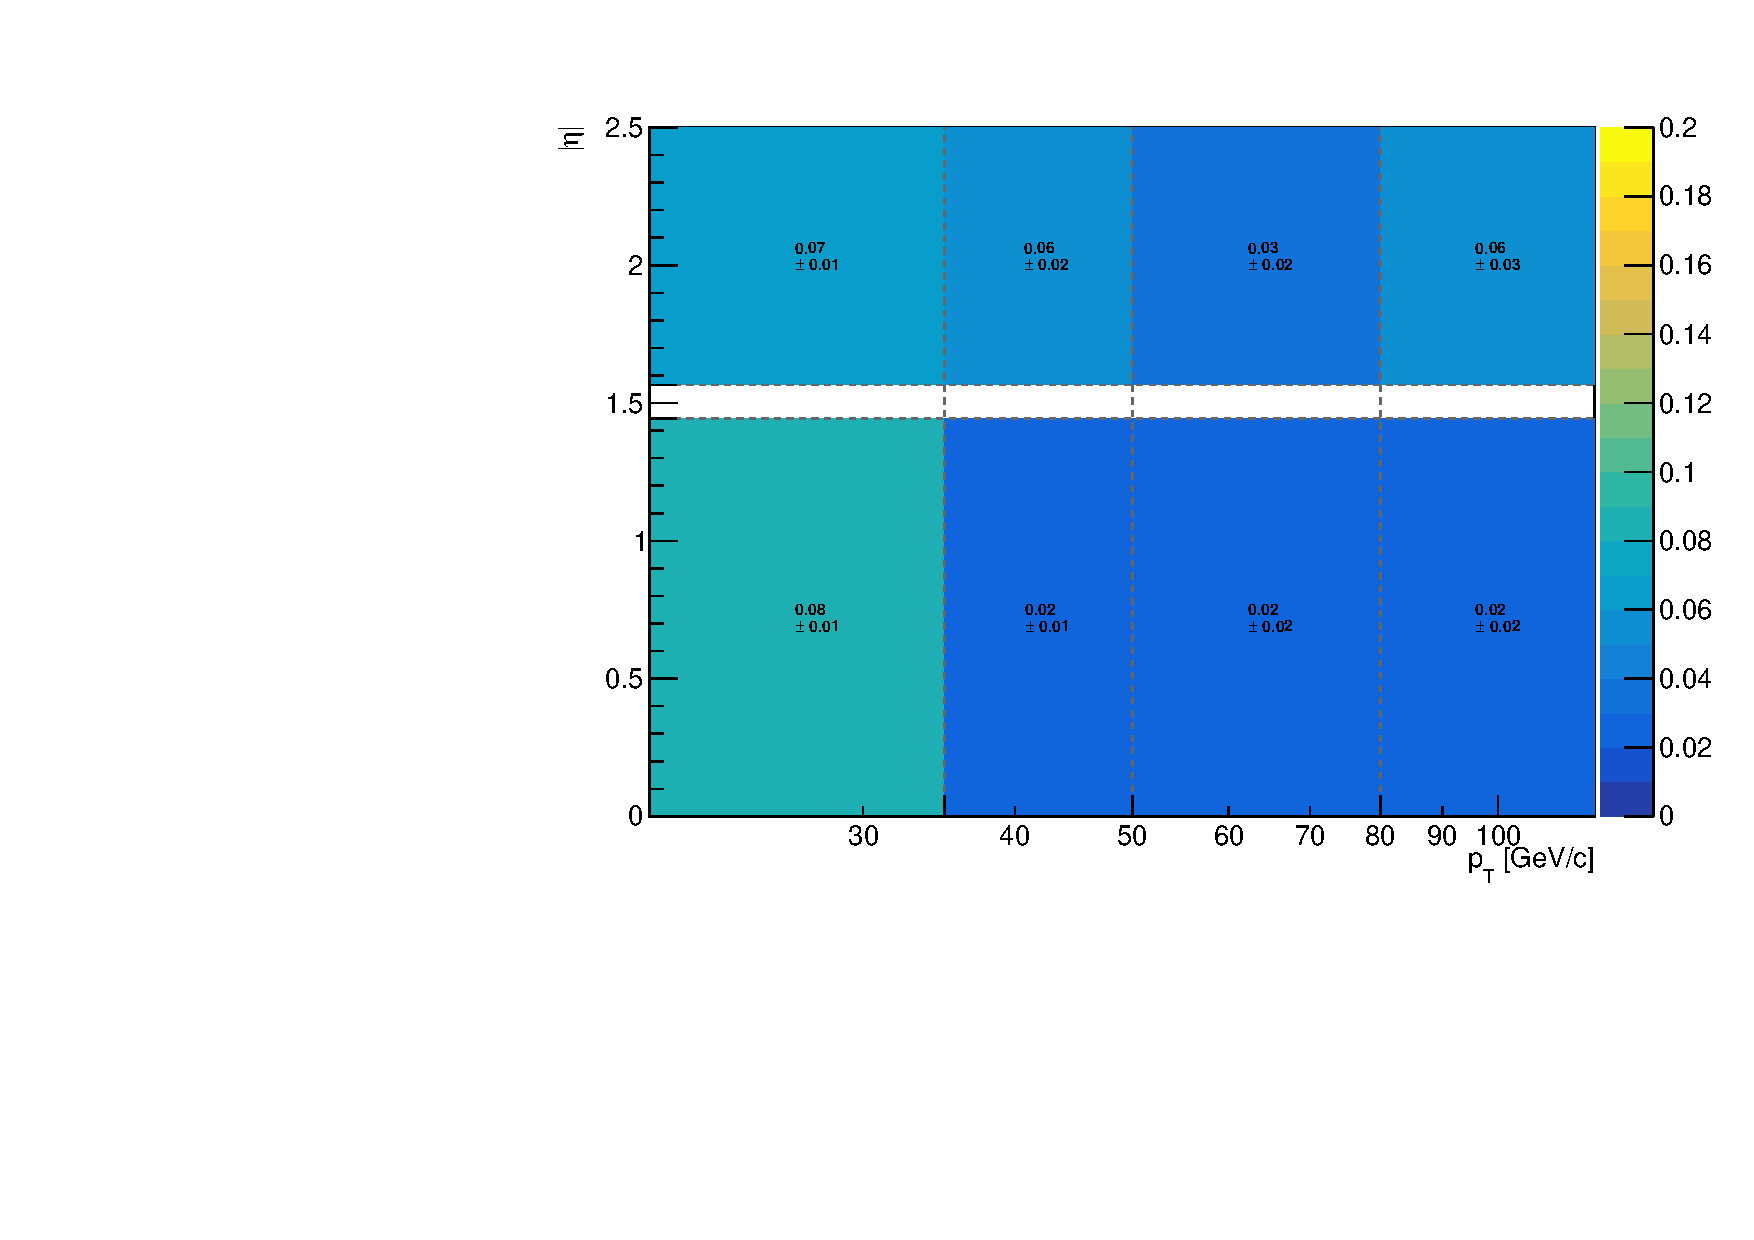
\includegraphics[width=.5\textwidth]{Figures/FR_VLtoL_pt-aeta_2x+e_data-ZGToLLG_2018.pdf}}}
\subfigure [$\ell^+ \ell^- \mu^\pm$] {\resizebox{.5\textwidth}{!}{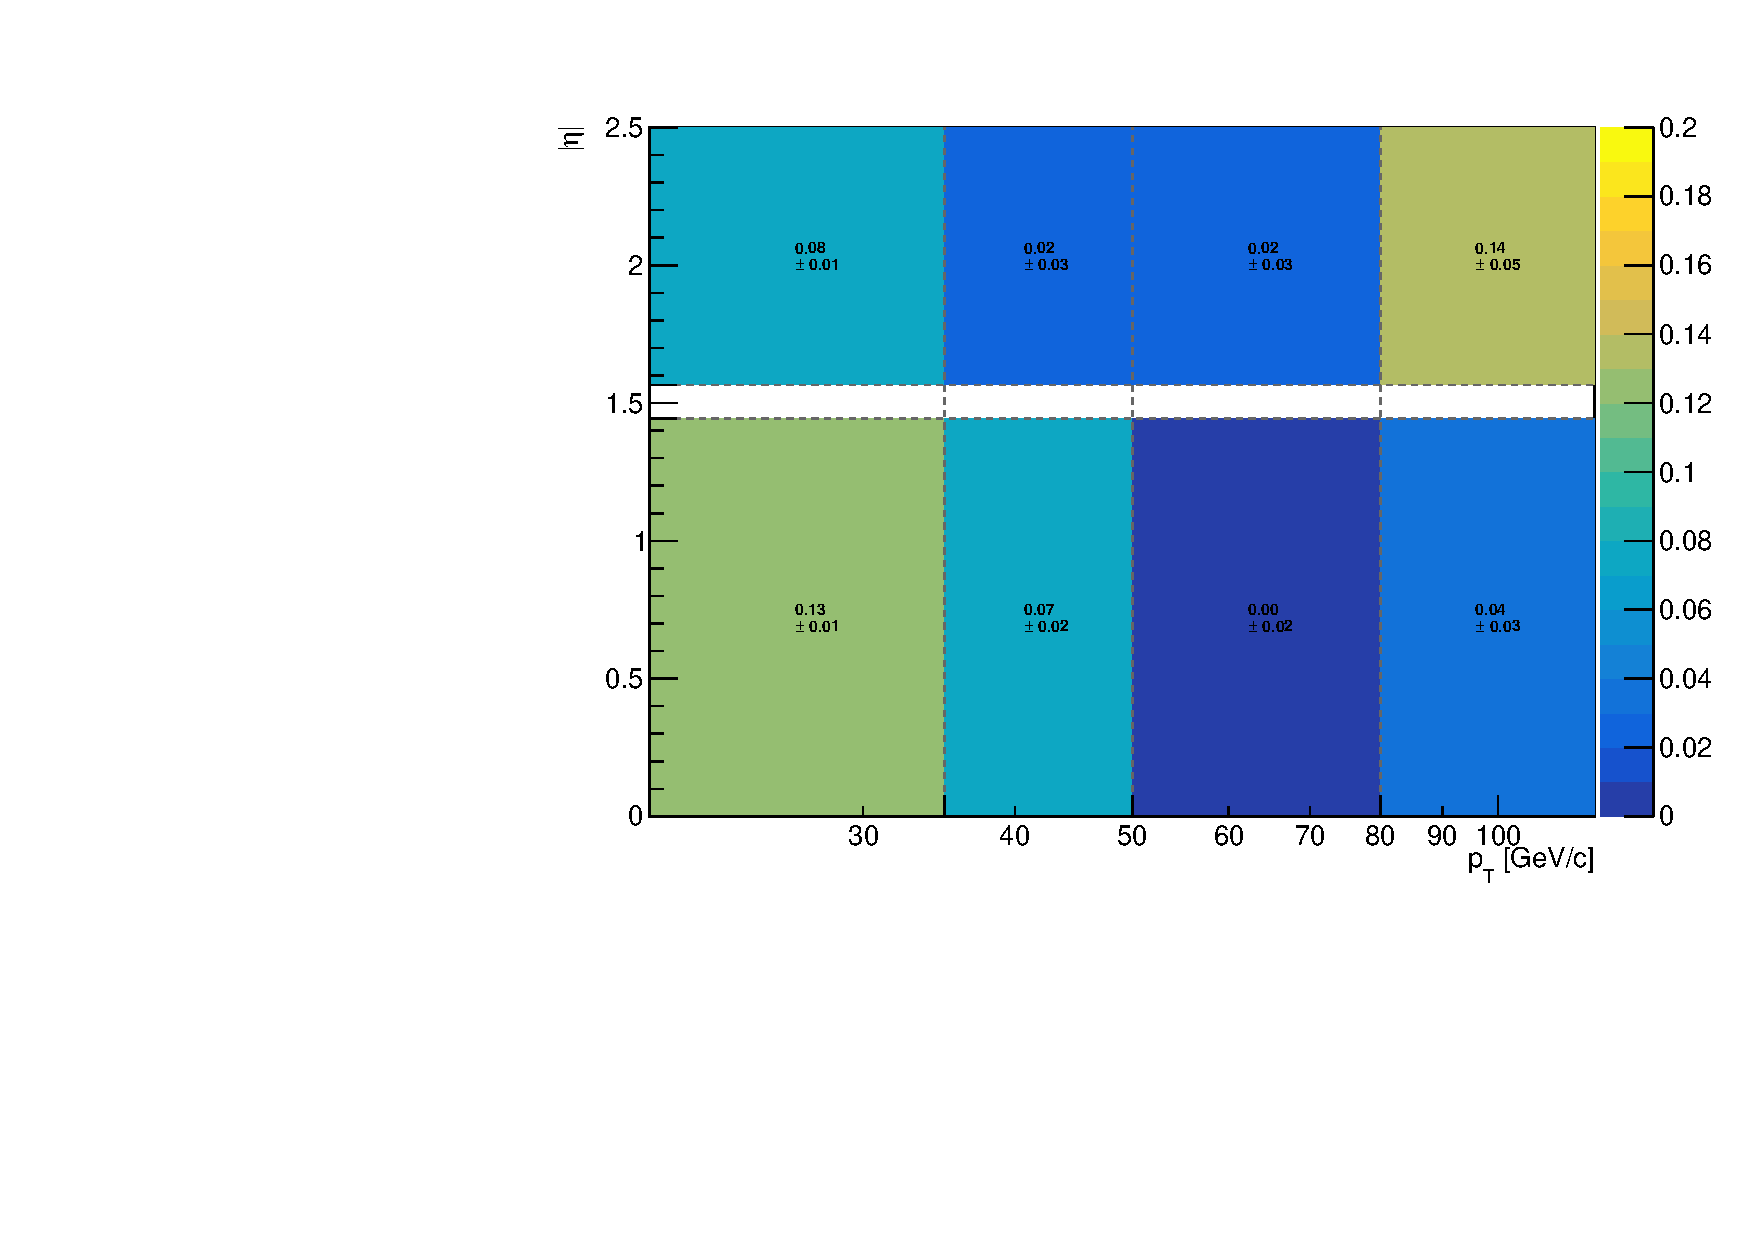
\includegraphics[width=.5\textwidth]{Figures/FR_VLtoL_pt-aeta_2x+m_data-ZGToLLG_2018.pdf}}}
\caption{Photon non-prompt rate as measured in 2018 data (with prompt $Z\gamma$ subtraction) in events with different flavours for the third lepton.}
\label{fig:phFR_em}
\end{figure}

Another test is performed by separating event where the third lepton passes/fails the tight analysis selection, shown in Figure \ref{fig:phFR_PF}.

\begin{figure}
\subfigure [$\ell^+ \ell^- \ell^\pm_{PASS}$] {\resizebox{.5\textwidth}{!}{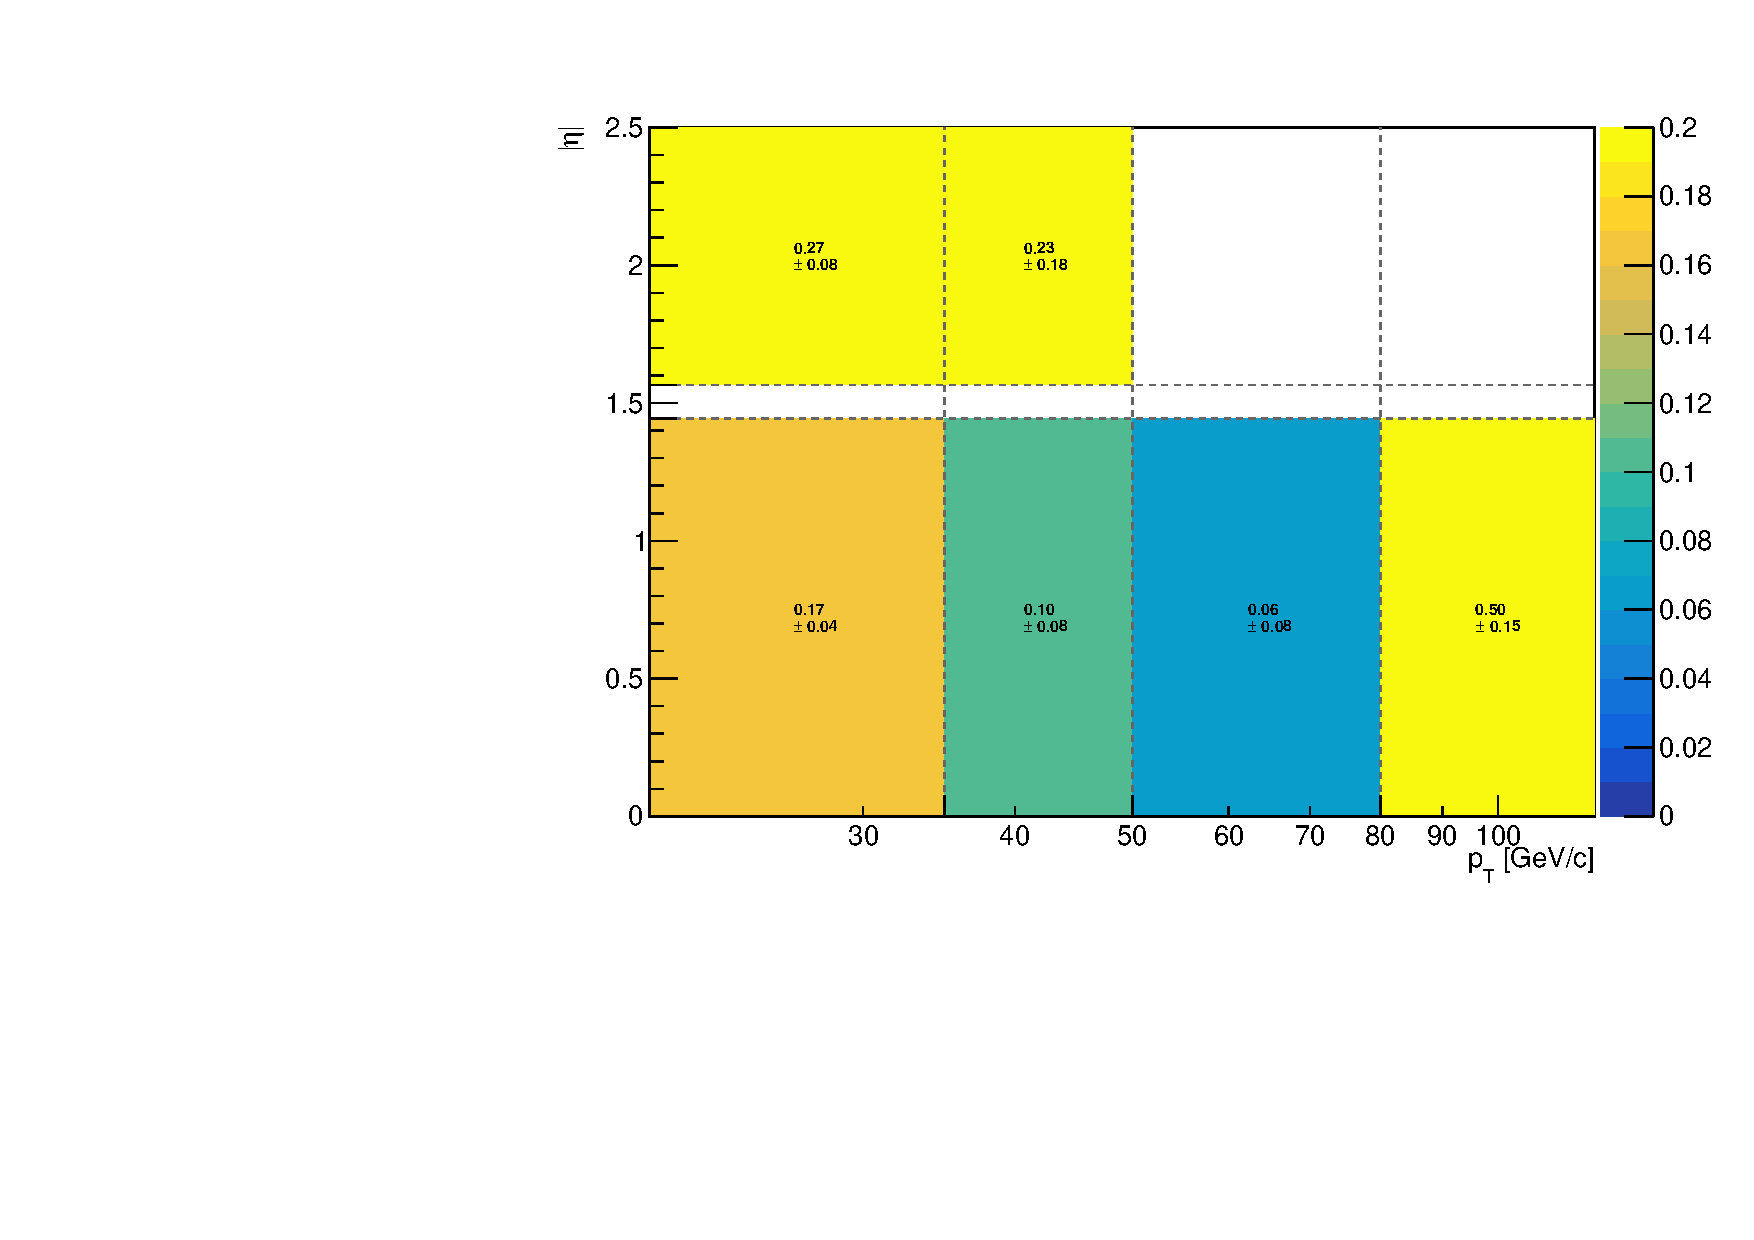
\includegraphics[width=.5\textwidth]{Figures/FR_VLtoL_pt-aeta_2x+P_data-ZGToLLG_2018.pdf}}}
\subfigure [$\ell^+ \ell^- \ell^\pm_{FAIL}$] {\resizebox{.5\textwidth}{!}{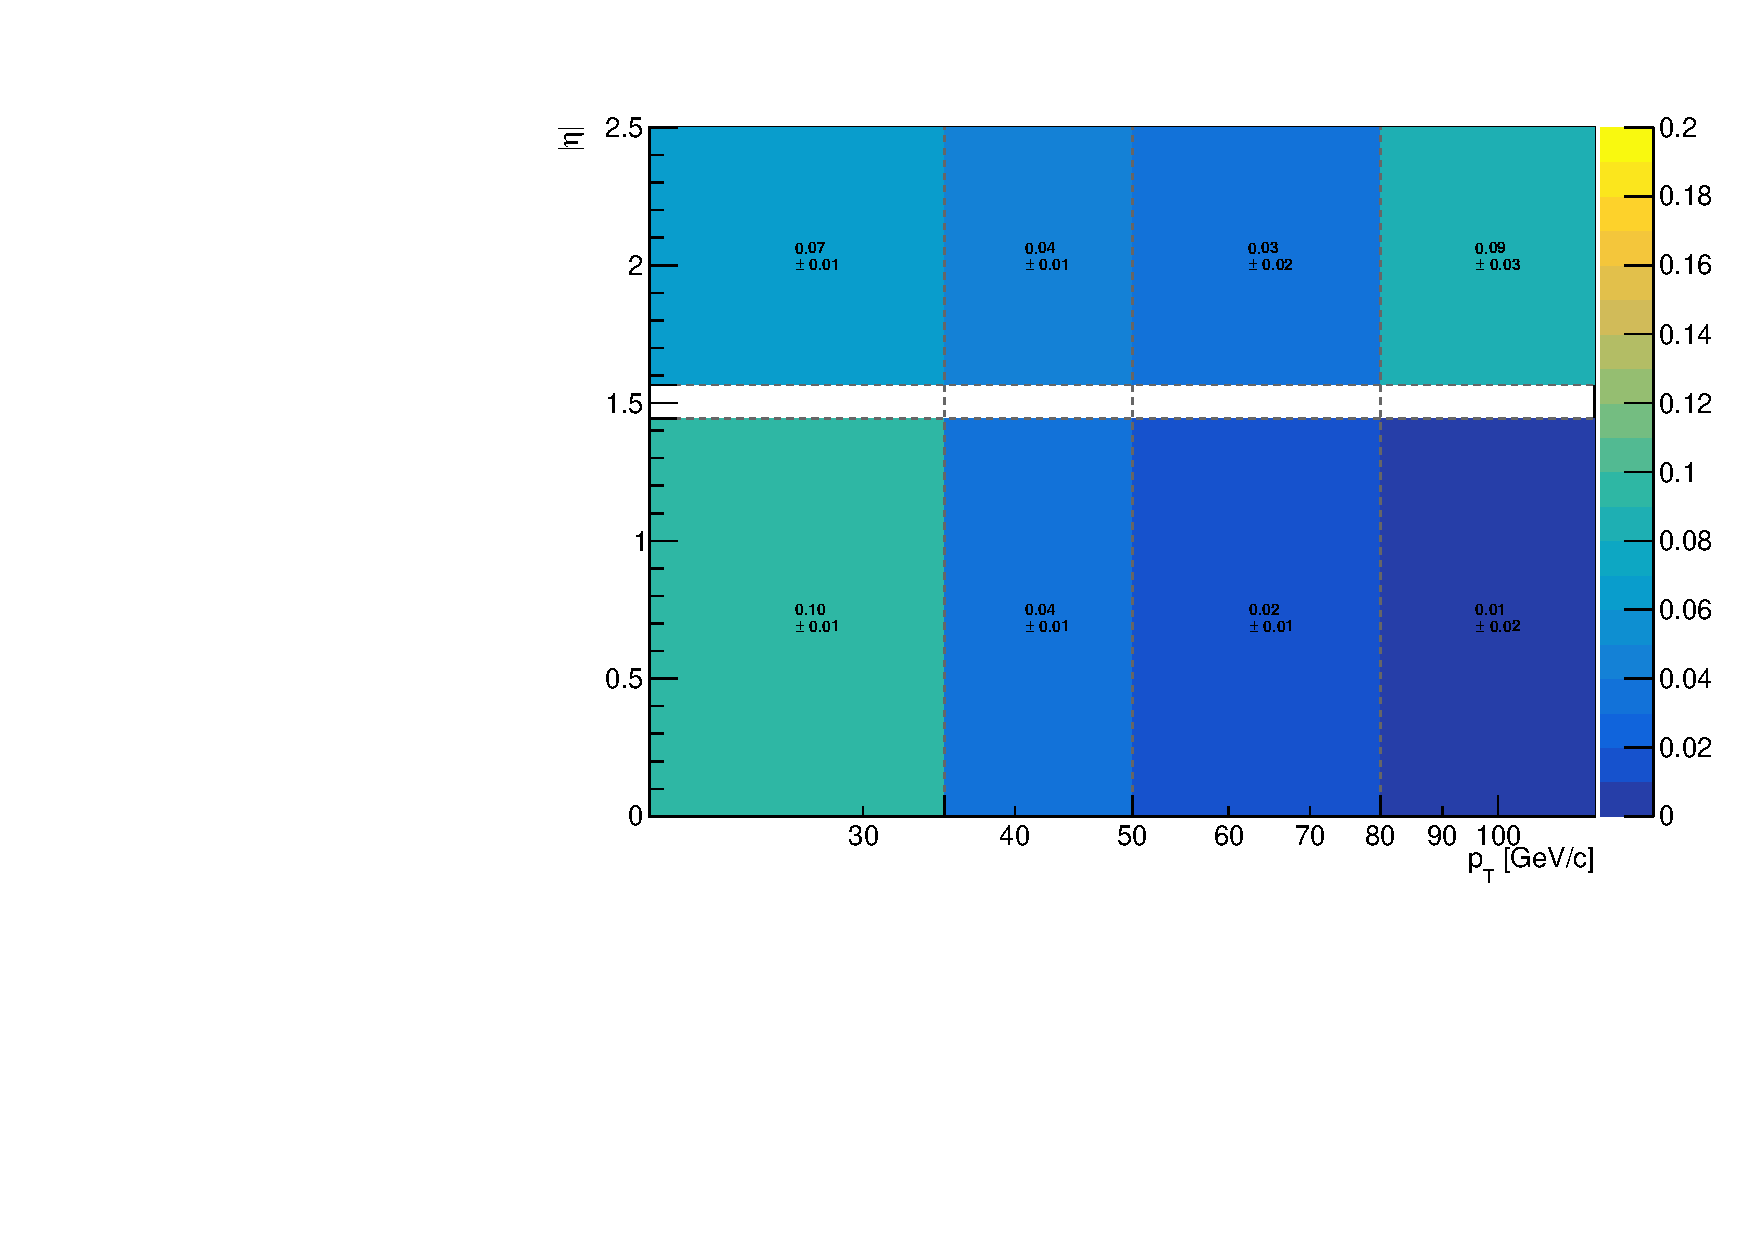
\includegraphics[width=.5\textwidth]{Figures/FR_VLtoL_pt-aeta_2x+F_data-ZGToLLG_2018.pdf}}}
\caption{Photon non-prompt rate as measured in 2018 data (with prompt $Z\gamma$ subtraction) in events where the third lepton passes/fails the tight selection, regardless of its flavour.}
\label{fig:phFR_PF}
\end{figure}

The trend for each $(p_{T}, |\eta|)$ bin for the different data-taking periods can be seen in Figure \ref{fig:phFR_time}.
It appears that, within the uncertainties, the measurements for each bin are compatible across the years and thus a single rate for the whole Run2 could be derived.

\begin{figure}
\centering
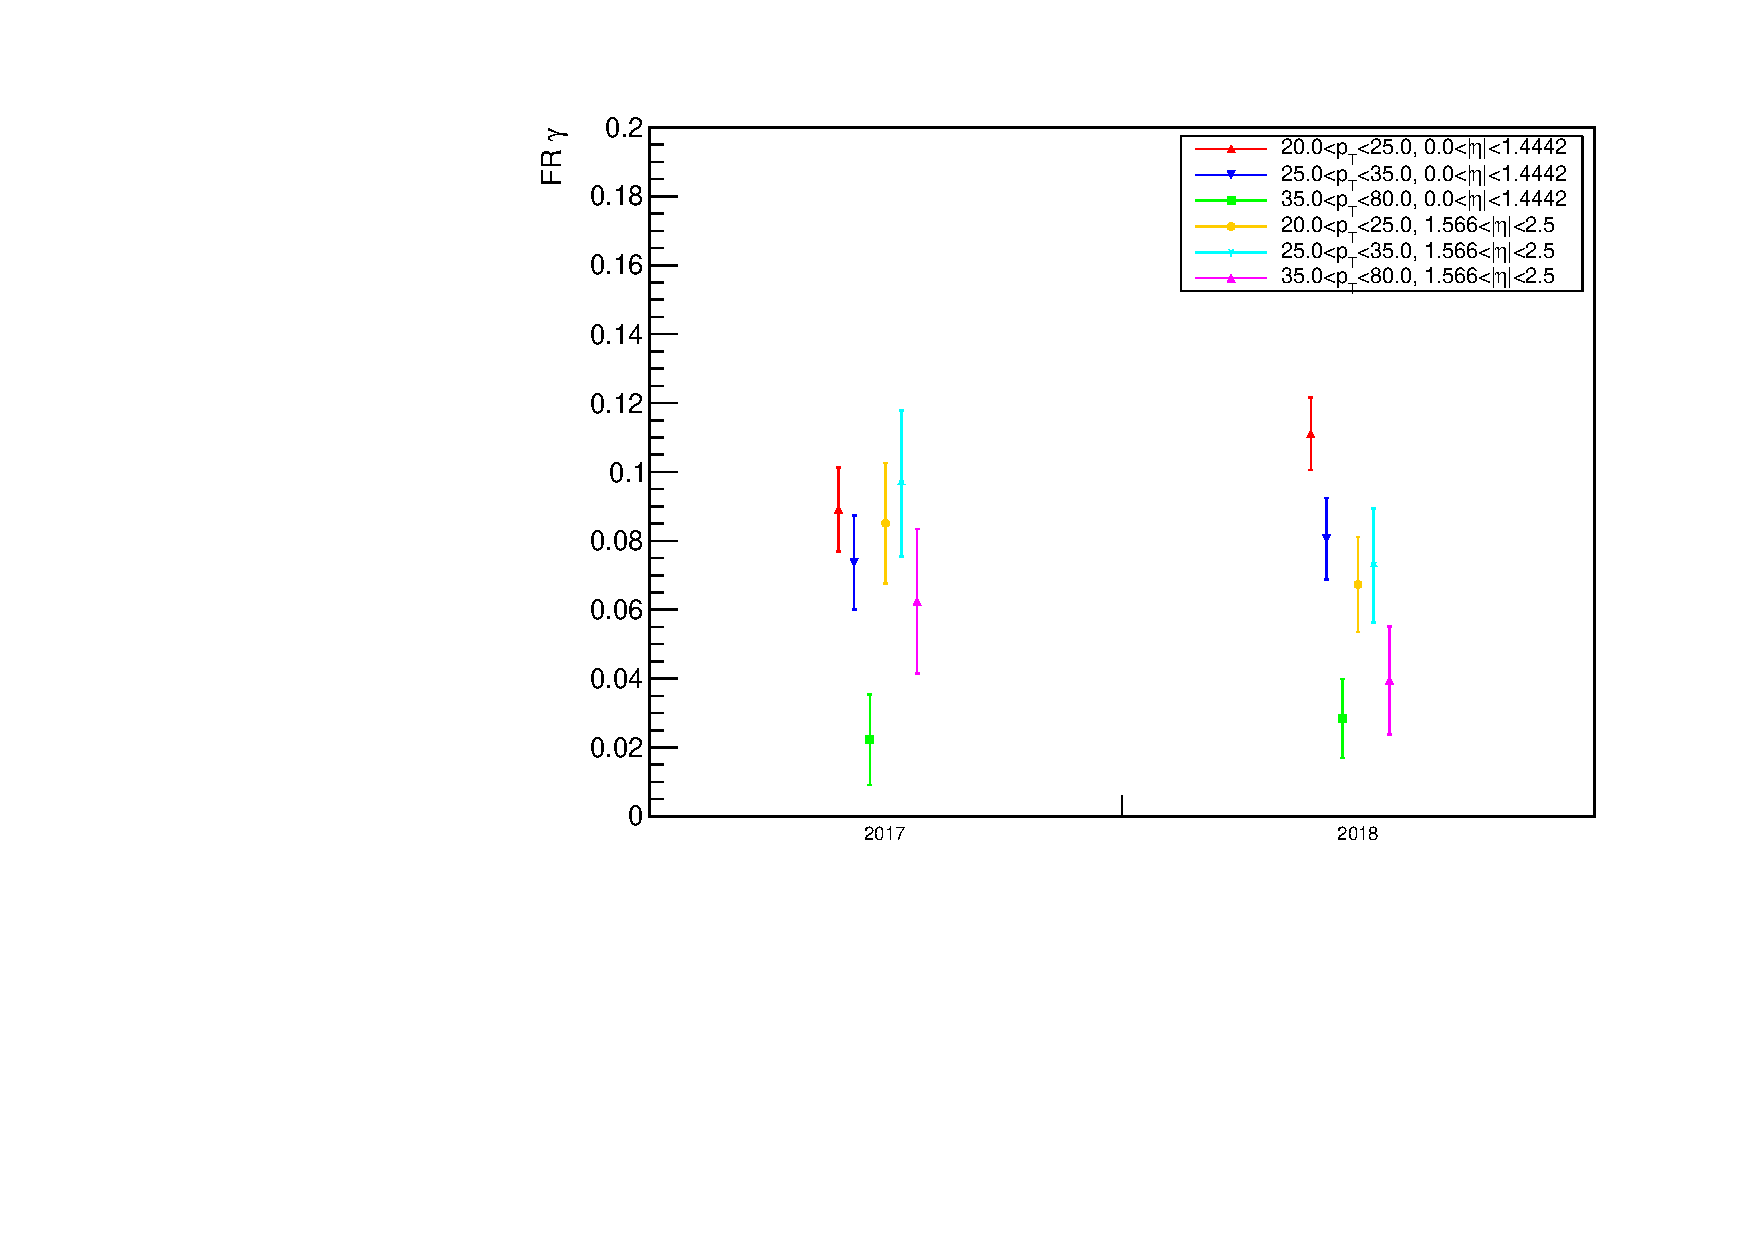
\includegraphics[width=.5\textwidth]{Figures/FR_VLtoL_pt-aeta_data-ZGToLLG_time.pdf}
\caption{Photon non-prompt rate in different data-taking periods.}
\label{fig:phFR_time}
\end{figure}

\subsubsection{Photon fake rate application}
The Fake Rate is then applied to events in the CR4P\_1F, CR3P\_1F and CR2P\_1F regions to estimate the non-prompt contribution in SR4P\_1P, SR3P\_1P, SR3P\_1P respectively.
Each event in this region is reweighed by the transfer factor $TF^\gamma(p_T, \eta) = \frac{f^\gamma}{1-f^\gamma}$, where $f^\gamma$ is the Fake Rate estimated in the measurement region.

\begin{equation}
  \begin{split}
    \label{eq:fakeRate_explanation_part1}
    N^{bkg}_{4P\_1P} &= \sum f_i N^{bkg}
    \\
    N^{bkg}_{4P\_1F} &= \sum ( 1-f_i ) N^{bkg}
  \end{split}
\end{equation}
where $N^{bkg}$ is the total number of events that have a fake photon, regardless of the region they are classified into.
From this it follows that the number of background events in the signal region is:
\begin{equation}
  \label{eq:fakeRate_explanation_part2}
  N^{bkg}_{4P\_1P} = \sum \frac{f_i}{1-f_i} N_{4P\_1F}
\end{equation}

\paragraph{Usage of the MVA based ID\\}
Additionally, kinematic photons that pass the MVA-based working points wp90 and wp80 are also considered,
given the improved performance of the MVA ID over the cut-based one.
The drawback is that this does not allow a data-driven estimation of the \nonprompt background,
due to the limited size of the application region defined by requiring a photon that passes the wp90 but fails the wp80.

Unlike a cut-based selection, it is not possible to invert only part of the MVA based ID.
The only way to derive a looser working point is to redo the optimisation of the raw MVA score,
and then study the efficiency of such selection in data and simulation to derive scale factors.
Both of these studies are outside the scope of this analysis.

Another possibility is to measure a fake rate between the kinematic selection and the looser MVA working point, \texttt{wp90}.
However, the former is too loose and the selected fakes have signatures that are very different from those of prompt photons.
This would make the assumption that the transfer factor is the same in the measurement and application regions quite unstable.

\todo{Add plots (e.g. Data/MC of CR3P1F/CR2P2F o SR4P blinded) of the number of events in wp90, wp80.}

Therefore, the results obtained using the MVA ID are derived without the data-driven estimate of fake photons.
In this case, the MC prediction of backgrounds which contain \nonprompt or misidentified photons is used.

\subsection{Final State Radiation}
\todo{TODO after discussion on ZZ and ZZgamma.}

\section{Dataset and samples}
\label{sec:datasets}

%% \subsection{CMS data}
This analysis uses a data sample recorded by the CMS experiment at a centre-of-mass energy of 13 \TeV during 2016, 2017 and 2018 corresponding to $\Lumi = 137 \fbinv$ of data.
Only data that passed the quality certification by all detector subsystems is used in the analysis.
%% and only luminosity sections included in the respective golden JSONs are used for further analysis.
The luminosity measurements are carried out by experts within the collaboration according to the metodology described in Ref. \cite{CMS:LUM-17-003}, for each year of data-taking \cite{CMS:LUM-17-004, CMS:LUM-18-002}.

The samples used correspond to the UltraLegacy reprocessing, which contains the most recent calibrations of all the physics objects reconstruction and identification criteria, as well as scale factors and uncertainties.
%% The MINIAOD format is chosen to perform the analysis.

The analysis relies on five different primary datasets (PD), 
{\it DoubleEG}, {\it DoubleMu}, {\it MuonEG}, {\it SingleElectron}, and {\it SingleMuon},
each of which combines a certain collections of HLT paths, whose exact requirements depend on the year of data 
taking. {\it DoubleEG} and {\it SingleElectron} are merged into {\it EGamma} in 2018.
To avoid duplicate events from different primary datasets, events are taken:

\begin{itemize}
\item from DoubleEG if they pass the diEle %(\texttt{HLT\_EleXX\_EleYY\_CaloIdXX\_TrackIdXX\_IsoXX(\_DZ)} )
  or triEle triggers, %(\texttt{HLT\_EleXX\_EleYY\_EleZZ\_CaloIdXX\_TrackIdXX}) where XX, YY and ZZ are year-dependent thresholds
\item from DoubleMuon if they pass the diMuon %(\texttt{HLT\_MuXX\_TrkIsoVVL\_MuYY\_TrkIsoVVL})
  or triMuon %(\texttt{HLT\_TripleMu\_XX\_YY\_ZZ})
  triggers and fail the diEle and triEle triggers,
\item from MuEG if they pass the MuEle %(\texttt{HLT\_MuXX\_TrkIsoXX\_EleYY\_CaloIdYY\_TrackIdYY\_IsoYY})
  or MuDiEle %(\texttt{HLT\_MuXX\_DiEleYY\_CaloIdYY\_TrackIdYY})
  or DiMuEle %(\texttt{HLT\_DiMuXX\_EleYY\_CaloIdYY\_TrackIdYY})
  triggers and fail the diEle, triEle, diMuon and triMuon triggers,
\item from SingleElectron if they pass the singleElectron trigger %(\texttt{HLT\_EleXX\_etaXX\_WPLoose/Tight(\_Gsf)})
  and fail all the above triggers.
\item from SingleMuon if they pass the singleMuon trigger %(\texttt{HLT\_IsoMuXX OR HLT\_IsoTkMuXX})
  and fail all the above triggers. 
\end{itemize} 

The used data sets are listed in Table~\ref{tab:datasamples}.%, along with the integrated luminosity.

\begin{table*}
  \caption{List of data samples used in the analysis. All runs for each of the 5 data streams are used, for a total of 76 primary datasets in the MINIAOD format.}
  \label{tab:datasamples}
  \centering
  \begin{tabular}{l l}
    \toprule
    \textbf{Data stream} &  \textbf{Run and reconstruction version}\\
    \midrule
    \multirow{9}{64pt}{%
      DoubleMuon\\
      DoubleEG\\
      MuonEG\\
      SingleMuon\\
      SingleElectron
    }&
    \multirow{9}{192pt}{%
      Run2016B-ver1\_HIPM\_UL2016\\
      Run2016B-ver2\_HIPM\_UL2016\\
      Run2016C-HIPM\_UL2016\\
      Run2016D-HIPM\_UL2016\\
      Run2016E-HIPM\_UL2016\\
      Run2016F-HIPM\_UL2016\\
      Run2016F-UL2016\\
      Run2016G-UL2016\\
      Run2016H-UL2016
    }
    \\
    \\
    \\
    \\
    \\
    \\
    \\
    \\
    \\
    \hline
    DoubleMuon     & Run2017B-UL2017\\
    DoubleEG       & Run2017C-UL2017\\
    MuonEG         & Run2017D-UL2017\\
    SingleMuon     & Run2017E-UL2017\\
    SingleElectron & Run2017F-UL2017\\
    \hline
    DoubleMuon & Run2018A-UL2018\\
    MuonEG     & Run2018B-UL2018\\
    SingleMuon & Run2018C-UL2018\\
    EGamma     & Run2018D-UL2018\\
    \bottomrule
  \end{tabular}
\end{table*}

%\begin{table}[h]
%\scriptsize
%    \centering
%    \begin{tabular}{l l l l} 
%\hline \hline%-----------------------------------------------------------------%---------------------------------------------------------
%HLT path                             & L1 seed        %                  & prescale  & primary dataset \\
%\hline %-----------------------------------------------------------------------%---------------------------------------------------
%\verb| HLT_Ele17_Ele12_CaloIdL_TrackIdL_IsoVL_DZ       | & \verb| L1_DoubleEG_15_10   |  & 1 & DoubleEG \\
%\verb| HLT_Ele23_Ele12_CaloIdL_TrackIdL_IsoVL_DZ       | & \verb| L1_DoubleEG_22_10   |  & 1 & DoubleEG \\
%\verb| HLT_DoubleEle33_CaloIdL_GsfTrkIdVL              | & \verb| (Multiple)          |  & 1 & DoubleEG \\
%\verb| HLT_Ele16_Ele12_Ele8_CaloIdL_TrackIdL           | & \verb| L1_TripleEG_14_10_8 |  & 1 & DoubleEG \\
%\verb| HLT_Mu17_TrkIsoVVL_Mu8_TrkIsoVVL                | & \verb| L1_DoubleMu_11_4    |  & 1 & DoubleMuon \\
%\verb| HLT_Mu17_TrkIsoVVL_TkMu8_TrkIsoVVL              | & \verb| L1_DoubleMu_11_4    |  & 1 & DoubleMuon \\
%\verb| HLT_TripleMu_12_10_5                            | & \verb| L1_TripleMu_5_5_3   |  & 1 & DoubleMuon \\
%\verb| HLT_Mu8_TrkIsoVVL_Ele17_CaloIdL_TrackIdL_IsoVL  | & \verb| L1_Mu5_EG15         |  & 1 & MuonEG \\
%\verb| HLT_Mu8_TrkIsoVVL_Ele23_CaloIdL_TrackIdL_IsoVL  | & \verb| L1_Mu5_EG20         |  & 1 & MuonEG \\
%\verb| HLT_Mu17_TrkIsoVVL_Ele12_CaloIdL_TrackIdL_IsoVL | & \verb| L1_Mu12_EG10        |  & 1 & MuonEG \\
%\verb| HLT_Mu23_TrkIsoVVL_Ele12_CaloIdL_TrackIdL_IsoVL | & \verb| L1_Mu20_EG10        |  & 1 & MuonEG \\
%\verb| HLT_Mu23_TrkIsoVVL_Ele8_CaloIdL_TrackIdL_IsoVL  | & \verb| L1_SingleMu*       |  & 1 & MuonEG \\
%\verb| HLT_Mu8_DiEle12_CaloIdL_TrackIdL                | & \verb| L1_Mu6_DoubleEG10   |  & 1 & MuonEG \\
%\verb| HLT_DiMu9_Ele9_CaloIdL_TrackIdL                 | & \verb| L1_DoubleMu7_EG7    |  & 1 & MuonEG \\
%\verb| HLT_Ele25_eta2p1_WPTight                        | & \verb| L1_SingleEG*         |  & 1 & SingleElectron \\
%\verb| HLT_Ele27_WPTight                               | & \verb| L1_SingleEG*         |  & 1 & SingleElectron \\
%\verb| HLT_Ele27_eta2p1_WPLoose_Gsf                    | & \verb| L1_SingleEG*         |  & 1 & SingleElectron \\
%\verb| HLT_IsoMu20 OR HLT_IsoTkMu20                    | & \verb| L1_SingleMu*         |  & 1 & SingleMuon \\
%\verb| HLT_IsoMu22 OR HLT_IsoTkMu22                    | & \verb| L1_SingleMu*         |  & 1 & SingleMuon \\
%\hline %--------------------------------------------------------------------------------------------------------------------------
%    \end{tabular}
%\small
%    \caption{Trigger paths used in this analysis.}% 2016 collision data.}
%    \label{tab:triggerPaths}
%\end{table}

\subsection{Simulation}
\texttt{MadGraph5\_aMCatNLO 2.6.2}~\cite{MGatNLO, Frederix_2018} is used to simulate the signal and most of the background contributions.
The simulation of $\PQq \PQq / \PQq \Pg \to \PZ \PZ \to 4 \Pl$ is done with \texttt{Powheg} \cite{Nason:2004rx, Frixione:2007vw, Alioli:2010xd, Alioli:2008gx},
while $\Pg \Pg \to \PZ \PZ \to 4 \Pl$ is simulated with \texttt{MCFM} \cite{MCFM}.
The simulation of the hadronization and parton shower is done by coupling the matrix element generators with \texttt{Pythia8} \cite{bierlich2022comprehensive, Sj_strand_2015} using the \texttt{CP5} tune \cite{CP5}.
The interaction of the particles with the CMS detector is simulated with \texttt{Geant4} \cite{GEANT}.

The MC samples are employed to optimize the event selection, evaluate the signal efficiency and acceptance, and optimise the search strategy for Triboson production.

\subsubsection{Signal}
The signal for this analysis is the production of a photon and two massive vector bosons, one of which is a $\Z$ that decays leptonically.
The hard process of the signal is simulated up to an additional jet at next to leading order (NLO) with FxFx merging.
Both of the fully leptonic signals ($\PZ\PZ\PGg \to 4\Pl\,\PGg$ and $\PW\PZ\PGg \to 3\Pl\,\PGn\,\PGg$)
are generated without forcing the intermediate vector boson resonances (e.g. \verb|p p > l+ l- l+ l- a|),
so as to retain and off-shell effects and spin correlations among the leptons in the final state.
Tau leptons are included in the generation, but are not part of the signal definition, and are suppressed in the analysis by the kinematic requirements on the Z mass.
No additional studies were conducted on the contamination of taus into the final state.

For the semileptonic signal samples ($\PZ\mathrm{V}\PGg \to 2\Pl\,2j\,\PGg$, $\mathrm{V} = W,\, Z$) an intermediate syntax is used,
with off-shell contributions for the leptonic decay of the \PZ,
while forcing the intermediate resonance for the hadronically decaying boson $\mathrm{V}$ (e.g. \verb|p p > z l+ l- a|).
The decays are performed by \texttt{MadSpin}~\cite{Artoisenet_2013}, in order to preserve the spin correlations between the leptons and, to some extent, off-shell effects.
The motivation of using the decay chain syntax is twofold, as it allows to speed up the generation and to populate the phase-space probed by the analysis.
The latter is crucial to ensure sufficient statistics.

\subsubsection{Background}
The dominant background for the three and four charged lepton final state are the production of $\PW\PZ$ and $\PZ\PZ$.
$\PW\PZ$ is simulated at NLO with MadGraph with up to 1 additional jet, including off-shell contributions.
%% $\PZ\PZ$ has contributions from $\PQq \PAQq \to \PZ\PZ$ and $\Pg \Pg \to \PZ\PZ$ (with a quark loop).

$\PQq \PAQq \to \PZ\PZ$ is simulated at NLO with Powheg up to one extra parton \todo{ask someone who knows if that's true},
using dynamical QCD factorization and renormalization scales.
Although the fully differential cross section has already been computed at NNLO \cite{},
this computation is not yet available in a Monte Carlo generator.

Aside from the dominant ZZ background mediated by the tree-level processes, there is also a gluon loop-induced ZZ production process,
which is a NNLO diagram and therefore is not included in the nominal ZZ sample.
Though suppressed by the two additional strong couplings, it nevertheless contributes to inclusive ZZ production at the 10\% level.
$\Pg \Pg \to \PZ\PZ$ is simulated, separately for the three final states 4\Pe, 2\Pe\PGm and 4\PGm, at LO with MCFM 7.0.

Rare backgrounds such as massive triboson VVV and $\PQt\PAQt \,+\, X$ are simulated at NLO with MadGraph5\_aMCatNLO.

%% The former is simulated at NLO with Powheg \todo{ask someone who knows if that's true},
%% while the latter is simulated with MCFM \todo{check how} separately for the three final states 4\Pe, 2\Pe\PGm and 4\PGm.

%% which are simulated at NLO up to 1-jet using MadGraph with FxFx merging.

% This LO sample is used for the development of the signal extraction MVA and the evaluation of the interference with the electroweak signal. It is not used in the statistical analysis of the VBS search, which uses the NLO FXFX sample described later.
%(only done in 2016) that only determines interference:
%include the electroweak and QCD as well as their interference:
%\begin{verbatim} 
%generate p p > z z j j QCD^2==2,  z  >  l+ l-
%\end{verbatim}
%The cross-sections reported by the generator with 2016 settings are reported in Table \ref{tab:signal_background_xsec}. It can be seen that the interference is positive and amounts to about 0.0426 fb or 10\% of the electroweak signal. The opposing kinematics of the QCD and electroweak production cause the interference to be concentrated in the same phase-space as the QCD background, as is shown in the tagging-jet mass $m_{jj}$ and $|\Delta\eta_{jj}|$ distribution in Fig.~\ref{fig:interference}. 
%The study of this sample is presented in the Appendix \ref{sec:interf}.
%\begin{table}[!h]
%\vspace{0.5cm}
%    \centering
%    \topcaption{Cross sections of the electroweak and QCD-induced production of the $4\ell jj$ final state and the interference. The phase space is that of the generation, i.e. $m_{jj}>100$~GeV and includes the branching ratios for the Z decays to electrons or muons.}
%   \begin{tabular}{c c c c c}
%   \hline \hline
%$\sigma_{QCD}$& $\sigma_{electroweak}$ & $\sigma_{sum} = \sigma_{QCD }+ \sigma_{electroweak}$ & $\sigma_{full}$ & $\sigma_{full} - \sigma_{sum}$\\
   
 %  \hline  
%9.335 fb& 0.4404 fb & 9.7754 fb & 9.818 fb & 0.0426 fb\\
%    \hline
%   \end{tabular}
%   \label{tab:signal_background_xsec}
%\end{table}
%\begin{figure}[!htb]
%\begin{center}
%    \subfigure [] {\resizebox{7.5cm}{!}{\includegraphics{Figures/interference_mjj}}}
%    \subfigure [] {\resizebox{7.5cm}{!}{\includegraphics{Figures/interference_deta.png}}}\\
%    \subfigure [] {\resizebox{10cm}{!}{\includegraphics{Figures/interference_bdt.png}}}
%\caption{
%Dijet invariant mass (left) and $|\Delta\eta|$ separation (right) distributions at GEN level for the electroweak signal, the QCD background and the interference between the two.
%}
%\label{fig:interference}
%\end{center}
%\end{figure}
% The MadGraph samples for signal and background do not include any decays to tau leptons. The expected yield of the tau final states (both $\ell^+\ell^-\tau^+\tau^-$ and $\tau^+\tau^-\tau^+\tau^-$) in the baseline selection (two on-shell Z bosons plus at least two jets with $m_{jj}>100$~GeV) is estimated using the MadGraph\_AMC@NLO FxFx 0,1 jet sample and is found to be 0.015~fb or 0.6\% of the total expected yield. This justifies not generating these final states in order to increase the statistics in the relevant lepton channels.
%The irreducible QCD-induced $\Pp\Pp  \to \Z\Z$ processes are produced at next-to-leading-order (NLO) with up to 2 extra parton emission with \texttt{MadGraph5\_aMCatNLO}~\cite{MGatNLO}, and merged using the FXFX scheme. This sample was specifically developed and requested for the ZZjj analysis; it will be the nominal sample in the statistical analysis.
%The jet multiplicities are generated separately, in order generate events in the phase space probed by this analysis: 
%\begin{verbatim} generate p p > z z j j  [QCD] \end{verbatim}
%The subsequent decays of the Z bosons to electrons or muons are performed in MadSpin, in order to preserve the spin correlations between the leptons. The FXFX merging scale $q_{cut} = 30\unit{GeV}$ as well as the minimum jet \pt cut $p_{T}^{jet}>15\unit{GeV}$ are identical to the values in the 0,1 jet FXFX sample.

The list of MC samples and their cross sections are shown in Table~\ref{tab:listofsamples}
and they include the ones detailed above as well as rare SM backgrounds that give much smaller background contributions.
%% For WZZ and ZZZ the dijet mass at LHE level has been required to be larger than 100 \GeV event by event, to avoid double counting with the signal sample.
All cross sections used in the analysis are those returned by the generator and reported in Table~\ref{tab:listofsamples}, with no additional k-factors being used.
The \texttt{PYTHIA 8}~\cite{Sjostrand:2015} package is used for parton showering, hadronization, and the underlying event simulation for all MC samples,
with parameters set by
%% the CUETP8M1 tune~\cite{CMS-SMP-12-016} (2016 data taking period) and
the CP5 tune~\cite{CP5}. %% (2017 and 2018 data taking periods).
All samples are generated with the NNPDF 3.0 (in 2016) or 3.1 (2017-18) parton distribution functions (PDFs)~\cite{NNPDF2015}.
The MC samples are reweighed based on the per-event true number of interactions to match the level of pileup observed in data as per general recipes.

% Figure \ref{fig:data_nvtx} shows the number of reconstructed vertices after the reweighing for 2016, similar figures are produced for 2017 and 2018.
%\begin{figure}[!htb]
%\vspace*{0.3cm}
%\begin{center}
%\includegraphics[width=0.55\textwidth]{Figures/data_mc_ZZ_Nvtx.pdf}
%\end{center}
%\caption{Number of reconstructed vertices in ZZ events with the pileup-reweighed MC. Fixme: check final cross section recommendation for reweighing.}
%\label{fig:data_nvtx}
%\end{figure}
% The default set of parton distribution functions (PDF) used for LO generators is \texttt{CTEQ6L}~\cite{CTEQ6L}, whereas \texttt{CT10}~\cite{CT10} is used for NLO generators (FIXME).
%Leptons are generated requiring  $m_{\ell^{+}\ell^{-}}> 4$ GeV in all samples but \texttt{MadGraph}, in which  $m_{\ell^{+}\ell^{-}} > 12$ GeV, and reconstructed  following the same steps of~\cite{HiggsLegacyPaper,ZZXSPaper}. Jets are generated with $p_{T} > 10$ GeV and reconstructed following the criteria recommended by Jet-MET group~\cite{JetID}.

\begin{sidewaystable}
  \caption{List of signal and background samples used in the analysis, with the Matrix Element generator used and their cross section.}
  \label{tab:listofsamples}
  \centering
  \resizebox{\textwidth}{!}{
  \begin{tabular}{l l r l m{.18\textwidth}}
    \toprule
    Process & Generator & Cross Section [pb] & Sample name & Remarks\\

    \midrule
    \multicolumn{5}{l}{Signal samples}\\
    \hline
    $\PZ\PZ\PGg \to 4\Pl\,\PGg$      & MadGraph (NLO) & 0.02202  & {\small\tt ZZGJetsTo4L2Nu\_4f\_TuneCP5\_13TeV\_amcatnloFXFX\_pythia8/[1,2,3,4]} &\\ %pp>l+ l- l+ l-a [QCD]; lep = e mu ta
    $\PW\PZ\PGg \to 3\Pl\,\PGn\,\PGg$& MadGraph (NLO) & 0.03844  & {\small\tt LLWA\_WToLNu\_4FS\_TuneCP5\_13TeV-amcatnlo-pythia8/[1,2,3,4]} &\\ %pp>lep nu z a [QCD]; lep = e mu ta
    $\PZ\PZ\PGg \to 2\Pl\,2j\,\PGg$  & MadGraph (NLO) & 0.04978  & {\small\tt ZTo2LZTo2JGToG\_TuneCP5\_13TeV\_amcatnloFXFX-pythia8/[1,2,3,4]} &\\
    $\PW\PZ\PGg \to 2\Pl\,2j\,\PGg$  & MadGraph (NLO) & 0.08044  & {\small\tt WTo2JZTo2LG\_TuneCP5\_13TeV-amcatnloFXFX-pythia8/[1,2,3,4]} &\\

    \midrule
    \multicolumn{5}{l}{Irreducible background samples}\\
    \hline
    $\PZ\PZ\to 4\Pl$ + 0,1 jets      & MadGraph (NLO) & 1.256    & {\small\tt ZZTo4L\_TuneCP5\_13TeV\_powheg\_pythia8/[1,2,3,4]}                    &\\
    $\Pg\Pg\to \PZ\PZ\to 4\PGm$      & MCFM (LO)      & 0.001586 & {\small\tt GluGluToContinToZZTo4mu\_13TeV\_TuneCP5\_MCFM701\_pythia8/[1,2,3,4]}  &\\
    $\Pg\Pg\to \PZ\PZ\to 4\Pe$       & MCFM (LO)      & 0.001586 & {\small\tt GluGluToContinToZZTo4e\_13TeV\_TuneCP5\_MCFM701\_pythia8/[1,2,3,4]}   &\\ 
    $\Pg\Pg\to \PZ\PZ\to 2\Pe\,2\PGm$& MCFM (LO)      & 0.003191 & {\small\tt GluGluToContinToZZTo2e2mu\_13TeV\_TuneCP5\_MCFM701\_pythia8/[1,2,3,4]}&\\

    \midrule
    \multicolumn{5}{l}{Reducible background samples}\\
    \hline
    $\PZ$ + 0,1,2 jets               & MadGraph (NLO) & 6225.2   & {\small\tt DYJetsToLL\_M-50\_TuneCP5\_13TeV-amcatnloFXFX-pythia8/[1,2,3,4]} & for data/MC comparison in Z+X CR\\% define lep+ = e+ mu+ ta+; generate p p > lep+ lep- j [QCD]; add process p p > lep+ lep- j j [QCD]
    $\PZ\PGg$ + 0,1 jets             & MadGraph (NLO) & 55.48    & {\small\tt ZGToLLG\_01J\_5f\_TuneCP5\_13TeV-amcatnloFXFX-pythia8/[1,2,3,4]} & for prompt \PGg subtraction in Z+X CR\\% define lep = e+ mu+ ta+ e- mu- ta-; generate p p > lep lep a [QCD]; add process p p > lep lep a j [QCD]
    $\PW\PZ \to 3\Pl\,\PGn$          & MadGraph (NLO) & 5.213    & {\small\tt WZJToLLLNu\_TuneCP5\_13TeV-amcnlo-pythia8/[1,2,3,4]}             & off-shell contrib., letptonic decays\\ % define p = p b b~; define j = j b b~; define ell+ = e+ mu+ ta+; generate p p > ell- vl~ ell+ ell- (+ h.c.); add process p p > ell- vl~ ell+ ell- j (+ h.c)
    $\PQt\PAQt \to 2\Pl\,PGn$ + jets & Powheg         & 87.3     & {\small\tt TTTo2L2Nu\_TuneCP5\_13TeV-powheg-pythia8/[1,2,3,4]}              &\\

    \midrule
    \multicolumn{5}{l}{Rare background samples}\\
    \hline
    $\PQt\PAQt\PZ$ + 0,1 jets        & MadGraph (LO)  & 0.5407   & {\small\tt ttZJets\_TuneCP5\_13TeV\_madgraphMLM\_pythia8]}  & inclusive \PZ decays\\
    $\PQt\PAQt\PW$ + 0,1 jets        & MadGraph (NLO) & 0.2161   & {\small\tt TTWJetsToLNu\_TuneCP5\_13TeV-amcatnloFXFX-madspin-pythia8/[1,2,3,4]}& p p > t t\~ l v\\
    $\PQt\PAQt\PZ\PZ$ + jets         & MadGraph (LO)  & 0.001572 & {\small\tt TTZZ\_TuneCP5\_13TeV-madgraph-pythia8/[1,2,3,4]} & inclusive decays\\
    $\PQt\PAQt\PW\PW$ + jets         & MadGraph (LO)  & 0.007883 & {\small\tt TTWW\_TuneCP5\_13TeV-madgraph-pythia8/[1,2,3,4]} & inclusive decays\\
    $\PZ\PZ\PZ$ + jets               & MadGraph (NLO) & 0.01398  & {\small\tt ZZZ\_TuneCP5\_13TeV-amcatnlo-pythia8/[1,2,3,4]}  & inclusive decays, $m_{jj}<100\GeV$\\
    $\PW\PZ\PZ$ + jets               & MadGraph (NLO) & 0.05565  & {\small\tt WZZ\_TuneCP5\_13TeV-amcatnlo-pythia8/[1,2,3,4]}  & inclusive decays, $m_{jj}<100\GeV$\\
    $\PW\PW\PZ$ + jets               & MadGraph (NLO) & 0.1651   & {\small\tt WWZ\_TuneCP5\_13TeV-amcatnlo-pythia8/[1,2,3,4]}  &\\
    $\PW\PW\PW$ + jets               & MadGraph (NLO) & 0.08058  & {\small\tt WWW\_4F\_TuneCP5\_13TeV-amcatnlo-pythia8/[1,2,3,4]}\\
    \bottomrule
    \\
    \multicolumn{5}{l}{[1] \texttt{RunIISummer20UL16MiniAODAPVv2-106X\_mcRun2\_asymptotic\_preVFP\_v*}}\\
    \multicolumn{5}{l}{[2] \texttt{RunIISummer20UL16MiniAODv2-106X\_mcRun2\_asymptotic\_v*}}\\
    \multicolumn{5}{l}{[3] \texttt{RunIISummer20UL17MiniAODv2-106X\_mc2017\_realistic\_v*}}\\
    \multicolumn{5}{l}{[4] \texttt{RunIISummer20UL18MiniAODv2-106X\_upgrade2018\_realistic\_v*}}\\
  \end{tabular}
  }
\end{sidewaystable}

\section{Event Selection}
\label{sec:event_selection}

\section{Fiducial region definition}
% the signal definition at gen level
The fiducial phase space definition mimics the selection described in Section \ref{sec:event_selection}.

The charged leptons, either electrons or muons are required to have $\pt > 5 \GeV$ and $|\eta| < 2.5$.
\todo{Each lepton pair $\Pl_i, \Pl_j$ must be separated $\DR(\Pl_i, \Pl_j) > 0.02$.}
\todo{Lepton isolation is ensured by requiring the scalar sum of the \pt of all stable particles, i.e.,
  those particles not decaying in the detector volume, within a cone of radius $\DR = 0.3$ to be less than 0.35 times the \pt of the lepton.}
Neutrinos, FSR photons, and leptons (electrons and muons) are not included in
the computation of the isolation sum to enhance the model independence of the measurements,
following the findings of Reference \cite{HIG-14-028}.
Low mass resonances are excluded by requiring that any opposite-sign lepton pair, regardless of flavour,
satisfies $m_{\Pl^{+} \Pl'^{-}} > 4\GeV$.

The number of charged leptons that pass these requirements is used to categorize the event into one of the three channels: 4\Pl, 3\Pl and 2\Pl.

The photon is required to have $\pt > 20 \GeV$, $|\eta| < 2.4$ and be produced in the hard scattering. % isPrompt
It must be separated from any lepton by $\DR(\PGg, \Pl) > 0.5$.

\todo{This paragraph is wrong.}
In the 2 \Pl channel, the two quarks from the decay of the VB must have $\pt > 30 \GeV$ and $|\eta| < 4.7$.
Their flavour must be compatible with a \PZ decay (e.g. \PQu\PAQu, \PQd\PAQd, \PQs\PAQs, \PQc\PAQc or \PQb\PAQb),
or a \PW decay (e.g. \PQu\PAQd, \PQu\PAQb, \PQd\PAQu, \PQd\PAQc, \PQs\PAQd or \PQs\PAQc).
The separation between the quarks and the photon must be $\DR(\PGg, \PQq) > 0.4$.
\todo{End of wrong}

In the 2 \Pl channel, jets are built with the \antikt algorithm with a distance parameter of 0.4,
and are required to have $\pt^{\rm jet} > 30 \GeV$ and $|\eta^{\rm jet}| < 4.7$, as done at the reconstruction level.
The jets are kept if no lepton or photon inside a cone with the size of the jet radius is found.

In the 4\Pl channel the leading (subleading) lepton must have \pt > 20 (10) \GeV.
There must be two pairs of same-flavour and opposite-sign (SFOS) leptons, which are labelled $\PZ_1$ and $\PZ_2$,
the former being the one with the mass closest the the Z peak, which must have $60 \GeV < m_{\PZ_{1,2}} < 120 \GeV$.

In the 3\Pl channel, the SFOS pair with the mass closest to the \PZ peak is selected first, and the remaining lepton is assigned to the \PW.
The mass of the \PZ boson must be $60 \GeV < m_\PZ < 120 \GeV$. %within 15 \GeV from the \PZ peak.
The leading (subleading) lepton from the \PZ boson must have \pt > 20 (10) \GeV,
while the lepton from the \PW must have \pt > 20 \GeV.

\section{Systematic uncertainties}
\label{sec:systematics}
The imperfect knowledge of the detector response and of the experimental conditions, as well as the limited precision of fixed-order theoretical calculations concur in increasing the uncertainty on the results.
The effects of these unknowns are accounted for as \textit{systematic uncertainties}, which are then included as nuisance parameter in the model used to perform the statistical analysis and extract the results (Section \ref{sec:statistical_analysis}).

The systematic uncertainties can have different effects.
\textit{Normalization} uncertainties affect the normalization of processes, changing the event yield.
\textit{Shape} uncertainties, in addition, modify the phisical observables (e.g. kinematics) of the events, and result in a different distribution of the event fraction in histogram bins.

Systematics can be divided, depending on their source, into \textit{theoretical} uncertainties, related to theory hypoteses and features of the numerical computations, and \textit{experimental} uncertainties, which depend on the knowledge of the detector response, running conditions, and include the data-driven estimation of backgound processes.
A detailed description of the various sources considered in this analysis follows.

\subsection{Theoretical uncertainties}
Theoretical uncertainties arise from the choice of the Parton Distribution Function (PDF) set,
the uncertainty on the strong coupling constant $\alpha_s$ and
the renormalization and factorization QCD scales, which account for the missing higher order uncertainty in finite order perturbative calculations.
All theoretical systematics act as normalization uncertainties and are correlated among data-taking periods

\subsection{Experimental uncertainties}
Experimental uncertainties have different sources.

The uncertainty on the integrated luminosity varies from 1.2 \% to 2.5 \% in the data-taking years, and the total uncertainty for Run 2 is 1.6 \%.
The luminosity measurements are carried out by experts within the collaboration according to the metodology described in Ref. \cite{CMS:LUM-17-003}, for each year of data-taking \cite{CMS:LUM-17-004, CMS:LUM-18-002}.

The uncertainty on lepton identification and reconstruction efficiency has an effect on the overall event yield ranging from 1 to 15 \% \todo{verify}.

The uncertanties coming from the data-driven estimation of fake lepton and fake photons backgrounds are also considered.
In both cases, the main contributions arise from the mismatch in background composition between the region in which the fake rate is measured and the regions where it its applied.
Additionally, in the case of the photon fake rate, the application region itself is statistically limited, and this introduces an additional uncertainty on the normalization of the fake photon process.


\begin{subappendices}
  \section{APV25 preamplifier saturation}
  \label{sec:APV}
In late 2015 and early 2016, the CMS strip tracker encountered a signal-to-noise ratio deterioration and a loss of hit detection on tracks, particularly as instantaneous luminosity increased.
Investigation revealed that the problem stemmed from saturation in the preamplifier of the strip readout chip (APV25) under high occupancies.
Lowering the operating temperature in \RunII{} unexpectedly prolonged preamplifier discharge time, resulting in charge buildup and a nonlinear response.
Muon reconstruction efficiency was also affected by preamplifier saturation.
%% The preamplifier's response was linear up to 3 MIPs, but nonlinear beyond.
This issue was resolved by adjusting the drain speed of the preamplifier~\cite{Butz:2018dum} through the preamplifier feedback voltage bias (VFP), achieving a recovery of the hit efficiency to the same level as in \Run1~\cite{CMS-TRK-20-001}.

A model for preamplifier saturation was developed and integrated into simulations, with adjustments yielding better data-model agreement.
As a consequence of these changes, for the year 2016, the detector simulations before and after the adjustment differ substantially.
The two periods, which correspond to luminosity of around 19.5 fb$^{-1}$ and 16.8 fb$^{-1}$,
are therefore analysed separately and are referred to as ``2016preVFP'' and ``2016postVFP''.

\end{subappendices}
